% I seguenti commenti speciali impostano:
% 1. 
% 2. PDFLaTeX come motore di composizione;
% 3. tesi.tex come documento principale;
% 4. il controllo ortografico italiano per l'editor.

% !TEX encoding = UTF-8
% !TEX TS-program = pdflatex
% !TEX root = tesi.tex
% !TEX spellcheck = it-IT

\documentclass[10pt,                    % corpo del font principale
               a4paper,                 % carta A4
               twoside,                 % impagina per fronte-retro
               openright,               % inizio capitoli a destra
               english,                 
               italian,                 
               ]{book}    

%**************************************************************
% Importazione package
%************************************************************** 

%\usepackage{amsmath,amssymb,amsthm}    % matematica

\usepackage[english, italian]{babel}    % per scrivere in italiano e in inglese;
                                        % l'ultima lingua (l'italiano) risulta predefinita

\usepackage{bookmark}                   % segnalibri

\usepackage{caption}                    % didascalie

\usepackage{chngpage,calc}              % centra il frontespizio

\usepackage{csquotes}                   % gestisce automaticamente i caratteri (")

\usepackage{emptypage}                  % pagine vuote senza testatina e piede di pagina

\usepackage{epigraph}			% per epigrafi

\usepackage{eurosym}                    % simbolo dell'euro

%\usepackage{indentfirst}               % rientra il primo paragrafo di ogni sezione

\usepackage{graphicx}                   % immagini

\usepackage{hyperref}                   % collegamenti ipertestuali

\usepackage[binding=5mm]{layaureo}      % margini ottimizzati per l'A4; rilegatura di 5 mm

\usepackage{listings}                   % codici

\usepackage{microtype}                  % microtipografia

\usepackage{mparhack,fixltx2e,relsize}  % finezze tipografiche

\usepackage{nameref}                    % visualizza nome dei riferimenti                                      

\usepackage[font=small]{quoting}        % citazioni

\usepackage{subfig}                     % sottofigure, sottotabelle

\usepackage[italian]{varioref}          % riferimenti completi della pagina

\usepackage[dvipsnames]{xcolor}         % colori

\usepackage{booktabs}                   % tabelle                                       
\usepackage{tabularx}                   % tabelle di larghezza prefissata                                    
\usepackage{longtable}                  % tabelle su più pagine                                        
\usepackage{ltxtable}                   % tabelle su più pagine e adattabili in larghezza

\usepackage[toc, acronym]{glossaries}   % glossario
                                        % per includerlo nel documento bisogna:
                                        % 1. compilare una prima volta tesi.tex;
                                        % 2. eseguire: makeindex -s tesi.ist -t tesi.glg -o tesi.gls tesi.glo
                                        % 3. eseguire: makeindex -s tesi.ist -t tesi.alg -o tesi.acr tesi.acn
                                        % 4. compilare due volte tesi.tex.

\usepackage[backend=biber,style=verbose-ibid,hyperref,backref]{biblatex}
                                        % eccellente pacchetto per la bibliografia; 
                                        % produce uno stile di citazione autore-anno; 
                                        % lo stile "numeric-comp" produce riferimenti numerici
                                        % per includerlo nel documento bisogna:
                                        % 1. compilare una prima volta tesi.tex;
                                        % 2. eseguire: biber tesi
                                        % 3. compilare ancora tesi.tex.

%**************************************************************
% file contenente le impostazioni della tesi
%**************************************************************

%**************************************************************
% Frontespizio
%**************************************************************

% Autore
\newcommand{\myName}{Alessandro Rizzo}                                    
\newcommand{\myTitle}{Studio e applicazione della \textit{Chaos Engineering} nello sviluppo di un microservizio reactive}

% Tipo di tesi                   
\newcommand{\myDegree}{Tesi di laurea}

% Università             
\newcommand{\myUni}{Università degli Studi di Padova}

% Facoltà       
\newcommand{\myFaculty}{Corso di Laurea in Informatica}

% Dipartimento
\newcommand{\myDepartment}{Dipartimento di Matematica "Tullio Levi-Civita"}

% Titolo del relatore
\newcommand{\profTitle}{Prof.ssa }

% Relatore
\newcommand{\myProf}{Silvia Crafa}

% Luogo
\newcommand{\myLocation}{Padova}

% Anno accademico
\newcommand{\myAA}{2019-2020}

% Data discussione
\newcommand{\myTime}{Settembre 2020}


%**************************************************************
% Impostazioni di impaginazione
% see: http://wwwcdf.pd.infn.it/AppuntiLinux/a2547.htm
%**************************************************************

\setlength{\parindent}{14pt}   % larghezza rientro della prima riga
\setlength{\parskip}{2pt}   % distanza tra i paragrafi


%**************************************************************
% Impostazioni di biblatex
%**************************************************************
\bibliography{bibliografia} % database di biblatex 

\defbibheading{bibliography} {
    \cleardoublepage
    \phantomsection 
    \addcontentsline{toc}{chapter}{\bibname}
    \chapter*{\bibname\markboth{\bibname}{\bibname}}
}

\setlength\bibitemsep{1.5\itemsep} % spazio tra entry

\DeclareBibliographyCategory{opere}
\DeclareBibliographyCategory{web}

\addtocategory{opere}{womak:lean-thinking}
\addtocategory{web}{site:agile-manifesto}

\defbibheading{opere}{\section*{Riferimenti bibliografici}}
\defbibheading{web}{\section*{Siti Web consultati}}


%**************************************************************
% Impostazioni di caption
%**************************************************************
\captionsetup{
    tableposition=top,
    figureposition=bottom,
    font=small,
    format=hang,
    labelfont=bf
}
%**************************************************************
% Impostazioni di glossaries
%**************************************************************

%**************************************************************
% Acronimi
%**************************************************************
\renewcommand{\acronymname}{Acronyms and abbreviations}

\newacronym[description={\glslink{iacg}{Infrastructure as Code}}]
    {iac}{IaC}{Inftrastructure as Code}


%**************************************************************
% Glossario
%**************************************************************
%\renewcommand{\glossaryname}{Glossario}

%\newglossaryentry{iacg}
%{
%    name=\glslink{iac}{IaC},
%    text=Infrastructure as Code,
%    sort=infrastructure as code,
%    description={Infrastructure as Code (IaC) is the managing and provisioning of infrastructure through code instead of through manual processes}
%}
%
%\newglossaryentry{Pulumi}
%{
%    name=\glslink{Pulumi}{pulumi},
%    text=Pulumi,
%    sort=pulumi,
%    description={Pulumi is}
%}

\newglossaryentry{cloud computing}
{
    name=\glslink{cloud computing}{cloud computing},
    text=cloud computing,
    sort=cloud computing,
    description={Cloud computing is on-demand access, via the internet, to computing resources—applications, servers (physical servers and virtual servers), data storage, development tools, networking capabilities, and more—hosted at a remote data center managed by a cloud services provider}
}

\newglossaryentry{cloud service provider}
{
    name=\glslink{cloud service provider}{cloud service provider},
    text=cloud service provider,
    sort=cloud service provider,
    description={Cloud service providers are companies that establish public clouds, manage private clouds, or offer on-demand cloud computing components (also known as cloud computing services) like Infrastructure-as-a-Service (IaaS), Platform-as-a-Service (PaaS), and Software-as-a-Service(SaaS). Cloud services can reduce business process costs when compared to on-premise IT}
}

\newglossaryentry{Terraform}
{
    name=\glslink{Terraform}{terraform},
    text=Terraform,
    sort=Terraform,
    description={Terraform is an open-source infrastructure as code (IaC) tool developed by HashiCorp. It allows developers to automate the creation, modification, and deletion of cloud resources in a scalable and efficient way }
}

\newglossaryentry{mixin-based composition}
{
    name=\glslink{mixin-based composition}{mixin-based composition},
    text=mixin-based composition,
    sort=mixin-based composition,
    description={In scala, trait mixins means you can extend any number of traits with a class or abstract class. You can extend only traits or combination of traits and class or traits and abstract class,
    Traits are used to share interfaces and fields between classes. They are similar to Java 8’s interfaces }
}

\newglossaryentry{AWS}
{
    name=\glslink{AWS}{aws},
    text=AWS,
    sort=AWS,
    description={AWS stands for Amazon Web Services. It is a comprehensive, evolving cloud computing platform provided by Amazon that includes a mixture of infrastructure-as-a-service (IaaS), platform-as-a-service (PaaS) and packaged-software-as-a-service (SaaS) offerings. AWS services can offer an organization tools such as compute power, database storage and content delivery services}
}


\newglossaryentry{EC2}
{
    name=\glslink{EC2}{EC2},
    text=EC2,
    sort=EC2,
    description={EC2 stands for elastic computing 2. EC2 is a module of AWS that provides scalable computing capacity in the Amazon Web Services (AWS) Cloud }
}

\newglossaryentry{JavaParser}
{
    name=\glslink{JavaParser}{Javaparser},
    text=JavaParser,
    sort=JavaParser,
    description={JavaParser is a Java library that provides you with an Abstract Syntax Tree of your Java code. The AST structure then allows you to work with your Java code in an easy programmatic way}
}

\newglossaryentry{sequence comprehension}
{
    name=\glslink{sequence comprehension}{sequence comprehension},
    text=sequence comprehension,
    sort=sequence comprehension,
    description={In Scala, a sequence comprehension is a syntactic construct that allows you to create new sequences by transforming and filtering existing ones. It's similar to a for loop in other languages, but with a more concise and functional syntax }
}

\newglossaryentry{Azure Resource Manager}
{
    name=\glslink{Azure Resource Manager}{Azure Resource Manager},
    text=Azure Resource Manager,
    sort=Azure Resource Manager,
    description={Azure Resource Manager is the deployment and management service for Azure. It provides a management layer that enables you to create, update, and delete resources in your Azure account
    }
}

\newglossaryentry{Azure}
{
    name=\glslink{Azure}{azure},
    text=Azure,
    sort=Azure,
    description={Microsoft Azure, formerly known as Windows Azure, is Microsoft's public cloud computing platform. It provides a broad range of cloud services, including compute, analytics, storage and networking}
}

\newglossaryentry{Cloud Deployment Manager}
{
    name=\glslink{Cloud Deployment Manager}{Cloud Deployment Manager},
    text=Cloud Deployment Manager,
    sort=Cloud Deployment Manager,
    description={Google Cloud Deployment Manager is an infrastructure deployment service that automates the creation and management of Google Cloud resources. Write flexible template and configuration files and use them to create deployments that have a variety of Google Cloud services, such as Cloud Storage, Compute Engine, and Cloud SQL, configured to work together}
}

\newglossaryentry{GCP}
{
    name=\glslink{GCP}{gcp},
    text=GCP,
    sort=GCP,
    description={Google Cloud Platform (GCP), offered by Google, is a suite of cloud computing services that runs on the same infrastructure that Google uses internally for its end-user products, such as Google Search, Gmail, Google Drive, and YouTube. Alongside a set of management tools, it provides a series of modular cloud services including computing, data storage, data analytics and machine learning}
}

\newglossaryentry{VPC}
{
    name=\glslink{VPC}{vpc},
    text=VPC,
    sort=VPC,
    description={A virtual private cloud (VPC) is a secure, isolated private cloud hosted within a public cloud. VPC customers can run code, store data, host websites, and do anything else they could do in an ordinary private cloud, but the private cloud is hosted remotely by a public cloud provider. (Not all private clouds are hosted in this fashion.) VPCs combine the scalability and convenience of public cloud computing with the data isolation of private cloud computing}
}

\newglossaryentry{subnet}
{
    name=\glslink{subnet}{Subnet},
    text=subnet,
    sort=subnet,
    description={In computer networking, a subnet is a smaller network within a larger network. It is created by dividing a larger network into smaller segments, with each segment having its own unique network address.\\
    A subnet is identified by its subnet mask, which is a 32-bit number used to divide an IP address into two parts - the network address and the host address. The subnet mask determines which bits in the IP address are used to identify the network and which bits are used to identify the hosts.\\
    Subnets are commonly used to improve network performance and security. By dividing a larger network into smaller subnets, network traffic can be reduced and more efficiently managed. Additionally, subnets can be used to isolate different parts of a network for security purposes, preventing unauthorized access to sensitive data or resources}
}

\newglossaryentry{internet gateway}
{
    name=\glslink{internet gateway}{internet gateway},
    text=internet gateway,
    sort=internet gateway,
    description={An internet gateway is a network component that serves as the entry and exit point between a private network, such as a Virtual Private Cloud (VPC) in the cloud, and the public internet.\\
    An internet gateway is responsible for translating the private IP addresses used within a private network to public IP addresses used on the internet, and vice versa. It enables instances within a VPC to communicate with the internet, and allows external users and resources to communicate with instances within the VPC.\\    
    An internet gateway typically includes two network interfaces - one that connects to the VPC, and another that connects to the public internet. It forwards traffic between the VPC and the internet, and routes traffic between the different subnets within the VPC}
}

\newglossaryentry{routing table}
{
    name=\glslink{routing table}{routing table},
    text=routing table,
    sort=routing table,
    description={In computer networking, a routing table, or routing information base (RIB), is a data table stored in a router or a network host that lists the routes to particular network destinations, and in some cases, metrics (distances) associated with those routes. The routing table contains information about the topology of the network immediately around it.\\
    In our case, the routing table has been used to bind the public subnets to the internet gateway, so that they can receive and send packets over the internet}
}

\newglossaryentry{abstract syntax tree}
{
    name=\glslink{abstract syntax tree}{AST},
    text=abstract syntax tree,
    sort=abstract syntax tree,
    description={In computer science, an abstract syntax tree (AST), or just syntax tree, is a tree representation of the abstract syntactic structure of text (often source code) written in a formal language. Each node of the tree denotes a construct occurring in the text}
} % database di termini
\makeglossaries


%**************************************************************
% Impostazioni di graphicx
%**************************************************************
\graphicspath{{immagini/}} % cartella dove sono riposte le immagini


%**************************************************************
% Impostazioni di hyperref
%**************************************************************
\hypersetup{
    %hyperfootnotes=false,
    %pdfpagelabels,
    %draft,	% = elimina tutti i link (utile per stampe in bianco e nero)
    colorlinks=true,
    linktocpage=true,
    pdfstartpage=1,
    pdfstartview=FitV,
    % decommenta la riga seguente per avere link in nero (per esempio per la stampa in bianco e nero)
    %colorlinks=false, linktocpage=false, pdfborder={0 0 0}, pdfstartpage=1, pdfstartview=FitV,
    breaklinks=true,
    pdfpagemode=UseNone,
    pageanchor=true,
    pdfpagemode=UseOutlines,
    plainpages=false,
    bookmarksnumbered,
    bookmarksopen=true,
    bookmarksopenlevel=1,
    hypertexnames=true,
    pdfhighlight=/O,
    %nesting=true,
    %frenchlinks,
    urlcolor=webbrown,
    linkcolor=RoyalBlue,
    citecolor=webgreen,
    %pagecolor=RoyalBlue,
    %urlcolor=Black, linkcolor=Black, citecolor=Black, %pagecolor=Black,
    pdftitle={\myTitle},
    pdfauthor={\textcopyright\ \myName, \myUni, \myFaculty},
    pdfsubject={},
    pdfkeywords={},
    pdfcreator={pdfLaTeX},
    pdfproducer={LaTeX}
}

%**************************************************************
% Impostazioni di itemize
%**************************************************************
\renewcommand{\labelitemi}{$\ast$}

%\renewcommand{\labelitemi}{$\bullet$}
%\renewcommand{\labelitemii}{$\cdot$}
%\renewcommand{\labelitemiii}{$\diamond$}
%\renewcommand{\labelitemiv}{$\ast$}


%**************************************************************
% Impostazioni di listings
%**************************************************************
\lstset{
    language=[LaTeX]Tex,%C++,
    keywordstyle=\color{RoyalBlue}, %\bfseries,
    basicstyle=\small\ttfamily,
    %identifierstyle=\color{NavyBlue},
    commentstyle=\color{Green}\ttfamily,
    stringstyle=\rmfamily,
    numbers=none, %left,%
    numberstyle=\scriptsize, %\tiny
    stepnumber=5,
    numbersep=8pt,
    showstringspaces=false,
    breaklines=true,
    frameround=ftff,
    frame=single
} 


%**************************************************************
% Impostazioni di xcolor
%**************************************************************
\definecolor{webgreen}{rgb}{0,.5,0}
\definecolor{webbrown}{rgb}{.6,0,0}


%**************************************************************
% Altro
%**************************************************************

\newcommand{\omissis}{[\dots\negthinspace]} % produce [...]

% eccezioni all'algoritmo di sillabazione
\hyphenation
{
    ma-cro-istru-zio-ne
    gi-ral-din
}

\newcommand{\sectionname}{sezione}
\addto\captionsitalian{\renewcommand{\figurename}{Figura}
                       \renewcommand{\tablename}{Tabella}}

\newcommand{\glsfirstoccur}{\ap{{[g]}}}

\newcommand{\intro}[1]{\emph{\textsf{#1}}}

%**************************************************************
% Environment per ``rischi''
%**************************************************************
\newcounter{riskcounter}                % define a counter
\setcounter{riskcounter}{0}             % set the counter to some initial value

%%%% Parameters
% #1: Title
\newenvironment{risk}[1]{
    \refstepcounter{riskcounter}        % increment counter
    \par \noindent                      % start new paragraph
    \textbf{\arabic{riskcounter}. #1}   % display the title before the 
                                        % content of the environment is displayed 
}{
    \par\medskip
}

\newcommand{\riskname}{Rischio}

\newcommand{\riskdescription}[1]{\textbf{\\Descrizione:} #1.}

\newcommand{\risksolution}[1]{\textbf{\\Soluzione:} #1.}

%**************************************************************
% Environment per ``use case''
%**************************************************************
\newcounter{usecasecounter}             % define a counter
\setcounter{usecasecounter}{0}          % set the counter to some initial value

%%%% Parameters
% #1: ID
% #2: Nome
\newenvironment{usecase}[2]{
    \renewcommand{\theusecasecounter}{\usecasename #1}  % this is where the display of 
                                                        % the counter is overwritten/modified
    \refstepcounter{usecasecounter}             % increment counter
    \vspace{10pt}
    \par \noindent                              % start new paragraph
    {\large \textbf{\usecasename #1: #2}}       % display the title before the 
                                                % content of the environment is displayed 
    \medskip
}{
    \medskip
}

\newcommand{\usecasename}{UC}

\newcommand{\usecaseactors}[1]{\textbf{\\Attori Principali:} #1. \vspace{4pt}}
\newcommand{\usecasepre}[1]{\textbf{\\Precondizioni:} #1. \vspace{4pt}}
\newcommand{\usecasedesc}[1]{\textbf{\\Descrizione:} #1. \vspace{4pt}}
\newcommand{\usecasepost}[1]{\textbf{\\Postcondizioni:} #1. \vspace{4pt}}
\newcommand{\usecasealt}[1]{\textbf{\\Scenario Alternativo:} #1. \vspace{4pt}}

%**************************************************************
% Environment per ``namespace description''
%**************************************************************

\newenvironment{namespacedesc}{
    \vspace{10pt}
    \par \noindent                              % start new paragraph
    \begin{description} 
}{
    \end{description}
    \medskip
}

\newcommand{\classdesc}[2]{\item[\textbf{#1:}] #2}
                     % file con le impostazioni personali

\begin{document}
%**************************************************************
% Materiale iniziale
%**************************************************************
\frontmatter
% !TEX encoding = UTF-8
% !TEX TS-program = pdflatex
% !TEX root = ../tesi.tex

%**************************************************************
% Frontespizio 
%**************************************************************
\begin{titlepage}

\begin{center}

\begin{LARGE}
\textbf{\myUni}\\
\end{LARGE}

\vspace{10pt}

\begin{Large}
\textsc{\myDepartment}\\
\end{Large}

\vspace{10pt}

\begin{large}
\textsc{\myFaculty}\\
\end{large}

\vspace{30pt}
\begin{figure}[htbp]
\begin{center}

\includegraphics[height=6cm]{logo-unipd}
\end{center}
\end{figure}
\vspace{30pt} 

\begin{LARGE}
\begin{center}
\textbf{\myTitle}\\
\end{center}
\end{LARGE}

\vspace{10pt} 

\begin{large}
\textsl{\myDegree}\\
\end{large}

\vspace{40pt} 

\begin{large}
\begin{flushleft}
\textit{Relatore}\\ 
\vspace{5pt} 
\profTitle \myProf
\end{flushleft}

\vspace{0pt} 

\begin{flushright}
\textit{Laureando}\\ 
\vspace{5pt} 
\myName
\end{flushright}
\end{large}

\vspace{40pt}

\line(1, 0){338} \\
\begin{normalsize}
\textsc{Anno Accademico \myAA}
\end{normalsize}

\end{center}
\end{titlepage} 
% !TEX encoding = UTF-8
% !TEX TS-program = pdflatex
% !TEX root = ../tesi.tex

%**************************************************************
% Colophon
%**************************************************************
\clearpage
\phantomsection
\thispagestyle{empty}

\hfill

\vfill

\noindent\myName: \textit{\myTitle,}
\myDegree,
\textcopyright\ \myTime.
% !TEX encoding = UTF-8
% !TEX TS-program = pdflatex
% !TEX root = ../tesi.tex

%**************************************************************
% Dedica
%**************************************************************
%\cleardoublepage
\phantomsection
\thispagestyle{empty}
\pdfbookmark{Dedica}{Dedica}

\vspace*{3cm}

\begin{center}
Dedicato alla mia famiglia e ai miei amici
\end{center}

% !TEX encoding = UTF-8
% !TEX TS-program = pdflatex
% !TEX root = ../tesi.tex

%**************************************************************
% Sommario
%**************************************************************
%\cleardoublepage
\phantomsection
\pdfbookmark{Sommario}{Sommario}
\begingroup
\let\clearpage\relax
\let\cleardoublepage\relax
\let\cleardoublepage\relax

\chapter{Abstract}

\intro{Scala as a candidate to address the problem of the always more complex management of the cloud infrastructure}\\
\newline
In the last decades the infrastructure used by companies changed deeply.
Years ago they were used to have on premise bare-metal servers, running their own applications, while now they rent cloud servers or applications and host their services in a serverless fashion.\\
Such a modern approach granted enormous benefits to flexibility, but at the same time greatly increased the complexity to manage the configuration of such infrastructures.
The current situation requires companies to resort to advanced tools for managing the always more complex structure of the owned cloud resources.
The critical aspects of such tools are the range of cloud service providers (AWS, Azure, ecc.) supported and the programming language offered to work with such tools.\\
Among all the tools that started to appear, Pulumi is the one that results to be the most innovative.
With its multi-cloud and multiple general programming languages support, has all the features to address the high requirements imposed by the more and more complex cloud scenario.\\
This thesis firstly shows why Scala represents an innovative addition to the Pulumi's current pool of supported languages.
Second, it also presents how a partial support for Scala has been smartly achieved using the Pulumi APIs of the already supported Java language and the interoperability between the various languages of the JVM.  %and how a partial support of the language has been achieved in a very limited time.
\newline
\newline
\newline
\newline
\newline
%The document describes the work done from the graduating Cisotto Emanuele, in collaboration with Zoleo Andrea, from the Kynetics Srl company.
%The objectives to achieve were many.\\
%First, the study of the basics of the functioning of the Pulumi technology and the Scala language was made.\\
%Second, a definition of a case study based on some \gls{AWS} \gls{EC2} resources was done. Hence, the respective implementation using Pulumi and the Typecript language has been done.\\
%Then, after having identified the shortcomings of Pulumi with the TypeScript language, a \textit{syntactic sugar} for the Scala support for Pulumi has been manually coded.
%Such a \textit{syntactic sugar} for Scala is based on the Java APIs for Pulumi.\\
%At that point, the same case study has been implemented with the newly created Scala APIs for Pulumi.\\
%Thus, an inspection of the Pulumi's Java libraries was made with the \gls{JavaParser} library, to infer useful information about the structure of the APIs so that an automatic generation of the \textit{syntactic sugar} code was possible.\\
%Finally, the code to automatically generate all the Scala \textit{syntactic sugar} code for all the AWS EC2 resources used in the case study was coded and used to generate such APIs.
%The generated code was eventually exported as a library so that it could be used in any Pulumi Scala project.




%\vfill
%
%\selectlanguage{english}
%\pdfbookmark{Abstract}{Abstract}
%\chapter*{Abstract}
%
%\selectlanguage{italian}

\endgroup			

\vfill


% !TEX encoding = UTF-8
% !TEX TS-program = pdflatex
% !TEX root = ../tesi.tex

%**************************************************************
% Ringraziamenti
%**************************************************************
%\cleardoublepage
\phantomsection
\pdfbookmark{Ringraziamenti}{ringraziamenti}

\begin{flushright}{
	\slshape    
	``Failures are a given, and everything will eventually fail over time''} \\ 
	\medskip
    --- Werner Vogels
\end{flushright}


\bigskip

\begingroup
\let\clearpage\relax
\let\cleardoublepage\relax
\let\cleardoublepage\relax

\chapter*{Ringraziamenti}
%\bigskip
\noindent \textit{Innanzitutto, vorrei esprimere la mia gratitudine alla Prof.ssa Silvia Crafa , relatrice della mia tesi, per la disponibilità e la cortesia mostratami durante quest'ultima parte del mio percorso.}\\

\noindent \textit{Desidero ringraziare Tiziano Campili che mi ha assistito durante lo \textit{stage} aziendale, in particolare per la sua disponibilità.}\\

\noindent \textit{Voglio ringraziare infine la mia famiglia e tutti i miei amici che mi sono stati vicini durante questo percorso accademico consigliandomi sempre per il meglio e senza lasciarmi mai solo.}\\


% \noindent\textit{\myLocation, \myTime}
% \hfill \myName

\endgroup


% !TEX encoding = UTF-8
% !TEX TS-program = pdflatex
% !TEX root = ../tesi.tex

%**************************************************************
% Indici
%**************************************************************
%\cleardoublepage
\pdfbookmark{\contentsname}{tableofcontents}
\setcounter{tocdepth}{3}
\tableofcontents
%\markboth{\contentsname}{\contentsname} 
\clearpage

\begingroup 
    \let\clearpage\relax
    \let\cleardoublepage\relax
    \let\cleardoublepage\relax
    %*******************************************************
    % Elenco delle figure
    %*******************************************************    
    \phantomsection
    \pdfbookmark{\listfigurename}{lof}
    \listoffigures

    \vspace*{8ex}

    %*******************************************************
    % Elenco delle tabelle
    %*******************************************************
    \phantomsection
    \pdfbookmark{\listtablename}{lot}
    \listoftables
        
    \vspace*{8ex}
\endgroup

\cleardoublepage

\cleardoublepage

%**************************************************************
% Materiale principale
%**************************************************************
\mainmatter          % Concept Preview}             
% !TEX encoding = UTF-8
% !TEX TS-program = pdflatex
% !TEX root = ../tesi.tex

%**************************************************************
\chapter{Introduction to Infrastructure as Code}
\label{cap:introduction-to-iac}
%**************************************************************

\intro{An introduction to IaC. The birth of the IaC is firstly presented, then the possible approaches, the advantages of using IaC, its challenges, and the evolution of the IaC with the second generation of tools}\\

%**************************************************************


\section{How we arrived to the IaC}
\label{sec:story-iac}

\subsection{Bare-metal servers and manual configurations}
Originally companies owned bare-metal servers on which hosted own services.
Each server was capable to host a single service.
The configuration of such servers was manually made using paper sheet with information about the configuration parameters (such as IPs, environment variables,etc.), or with shell scripts that had to be manually maintained and changed as the infrastructure changed or had to be reconfigured.
Some templates have been created to slightly automate the process of reconfiguration of the servers.\\

\subsection{The advent of the virtualization}
The virtualization era began as the virtual machine concept was born.
Here companies still had to own bare-metal servers, but the virtualization granted the possibility to scale software services upon one or more hardware servers.
This was possible to the decoupling between the hardware and the software.
However, to achieve this goal a further amount of configuration was required to be given and maintained.
The virtualization layer is having its own configuration, on top of the one of the bare-metal server.\\

\subsection{The cloud}
For a company, buying its own hardware servers have an extremely high cost at the beginning.
With the virtualization, the possibility to borrow hardware servers was made possible.
The virtual machines of the company are run on the rent servers thanks to the virtualization.
These operations were made possible by the management console offered by the providers of the servers, that allowed to instantiate the application as a virtual machine on their server.\\
With this cloud service providers were born, offering the bare-metal server rental service with a pay as you go pricing.
These borrowed machines compose the concept of \textit{cloud}.
The more resources you use (or rent), the more you pay.
Such an approach zeroes the initial costs to both buy, setup, and maintain a personal infrastructure.\\
Obviously this led to the need of having configuration files to ensure repeatability and reproducibility of the operations done on the cloud.
The engine that interprets such  files is host on the cloud itself.\\
At the same time, the APIs used from the management consoles have been exposed as official automation APIs.
We'll see soon how such APIs have a critical role in the IaC scenario.

\subsection{Towards the serverless}
A further step in the virtualization scenario has been achieved when the concept of container was born.
Before containers, whole virtual machines were being run on the virtual servers.
In most of the cases, the virtualization of the whole operative system (OS) of the virtual machine was an extra useless overhead.
The containers permitted to instantiate a virtual instance of service or application without the extra overhead of the OS.\\
Along with the concept of container also the container orchestration was born.
Such services allow containers to inter-operate.
In fact, the fact that containers contain single applications or services, they will likely need to communicate with each other.
Kubernetes for example, a container orchestration tool, is allowing to configure the interfaces to let containers communicate to each other.

\subsection{Serverless trend}
The most common applications started to be directly provided by the cloud service providers.
At this point, the user didn't have any more to take care of virtualizing a virtual machine or a container on a specific server.
He just had to request for the desired resource to the cloud provider and it would have taken care to virtualize it on an available machine (that could have been different any time the service was to be made available).\\
With this trend, also smaller custom logic started to be executed on virtual servers, such as custom lambdas, queues of messages, cache memory services, etc.\\
The serverless advent put even more pressure on the configuration required for the infrastructure.

\subsection{The advent of the Infrastructure as Code}
We notice from the previous paragraphs that, over time, the amount of configuration required has kept increasing over time, reaching its peak with the current serverless cloud scenario.
The necessity of configuration management tools was becoming real to keep up with the increasing complexity of the cloud structure and functioning.\\
With the advent of such tools, the Infrastructure as Code was born.
%It can be referred as the engineering of system administration activities


\section{Infrastructure as Code}

\subsection{What is IaC}
The evolution we have seen before has brought to an engineering of the system administration operations.
The management of configuration files for the infrastructure as code is at the base of the Infrastructure as Code (and here is why it is called so).
%It can't exist IaC without the IaaS (Infrastructure as a Service) concept.
%An IaaS is identified by set of raw IT resources offered to the user by the cloud service provider. They can be used to virtualise an infrastructure, or for resource-intensive projects — i.e. machine learning, big data, hosting, etc.\\
In other words, we could call Infrastructure as Code the process of managing and provisioning \gls{IaaS}s through machine-readable definition files, rather than physical hardware configuration or interactive configuration tools. \\
The IT infrastructure managed by this process comprises, as we have seen in the previous section, both physical equipment, such as bare-metal servers, and also virtual machines, virtualized applications and services, and the associated configuration resources. \\
The definitions may be in a version control system. The code in the definition files may use either scripts or declarative definitions, rather than maintaining the code through manual processes, but IaC more often employs declarative approaches.


\subsubsection{Types of approaches}

There are generally two approaches to IaC: declarative (functional) vs imperative (procedural). The difference between the declarative and the imperative approach is essentially \textit{what} versus \textit{how}.
The declarative approach focuses on what the eventual target configuration should be; the imperative focuses on how the infrastructure is to be changed to meet this.
The declarative approach defines the desired state and the system executes what needs to happen to achieve that desired state.
Imperative defines specific commands that need to be executed in the appropriate order to end with the desired conclusion.\\
In the \hyperref[sec:story-iac]{How we arrived to the IaC} section we have seen how first the APIs of the cloud service providers have been exposed, and only after the configuration management tools were born.
The exposed APIs are by nature imperative. In fact their usage is cumbersome and the user must be aware of what he is actually doing, otherwise configuration errors might happen.\\
The configuration management tools that were born after the serverless scenario arrived, are instead using a declarative approach.

\subsubsection{Methods}

There are two methods of IaC: push and pull.
The main difference is the manner in which the servers are told how to be configured.
In the pull method, the server to be configured will pull its configuration from the controlling server.
In the push method, the controlling server pushes the configuration to the destination system.

\subsection{Infrastructure as Code tools' main parts and their functioning}
From now on, for the aim of this thesis, with IaC tools we'll be referring to set of the following technologies: \gls{GCP}, \gls{Azure}, \gls{CloudFormation}, \gls{Terraform}, \gls{CDK}, and Pulumi.\\
The various existing IaC tools have a different architectures and functioning, but at their base they share the same abstract structure:
\begin{description}
  \item[declarative APIs for the user] these APIs let the user declare the resources that he would like to instantiate on a certain cloud service provider
  \item[backend engine] this engine will look at the resources declared by the user through the user APIs and will convert such declarations to REST API calls to the cloud service provider to instantiate them 
\end{description}
Obviously each tool has its own much more deep functioning.
We'll see how Pulumi works in the \hyperref[sec:pulumi-functioning]{Pulumi functioning} section.

%\subsubsection{IaC tool components}

%\paragraph{IaaS}
%The various cloud service providers (Amazon's \gls{AWS}, Microsoft's \gls{Azure}, Google's \gls{GCP}) let us define an Infrastructure as a Service, that is the base upon which the IaC lies.
%The IaaS-enabled cloud hosting platform offers APIs that allow users to automatically create, delete, and modify infrastructure resources on demand.

%\paragraph{Configuration Management platforms}
%The second main block of the Infrastructure as Code are the \textit{configuration management platforms} (CMP).
%Such a platform is a tools suite that connects to the IaaS APIs and automates common tasks.
%\gls{Terraform} and Pulumi are two examples of the currently present CMPs.
%The APIs exposed from the IaaS can be accessed by our CMP to automate the creation, deletion and update of the resources hosted on the cloud service provider.
%The resources states are defined by the user on a file which can either be based on a scripting language or on a general purpose programming language.
%Being code, the configuration files can be versioned, shared, and tested.

%\subsubsection{IaC workflow}
%A common workflow for any IaC tool of platform is here described:\\
%\begin{itemize}
%  \item first, the desired infrastructure resources to be created are declared in a file inside an application managed by a CMP
%  \item second, the engine of the CMP will execute the application, or inspect the resources declared in the file, and call the cloud service provider APIs to align the state of the cloud resources to the state defined in the user's file.
%\end{itemize}\mbox{}\\
%Obviously each tool has its own much more deep functioning.
%We'll see how Pulumi works in the \hyperref[sec:pulumi-functioning]{Pulumi functioning} section.




\subsection{Advantages of IaC}

The value of IaC can be broken down into three measurable categories: \textbf{cost}, \textbf{speed}, and \textbf{risk}.
Cost reduction aims at helping not only the enterprise financially, but also in terms of people and effort, meaning that by removing the manual component, people are able to refocus their efforts on other enterprise tasks.
Infrastructure automation enables speed through faster execution when configuring your infrastructure and aims at providing visibility to help other teams across the enterprise work quickly and more efficiently.
Automation removes the risk associated with human error, like manual misconfiguration; removing this can decrease downtime and increase reliability.\\
Related to the risk, we could highlight the importance of the \textbf{consistency} of such an approach.
Through the manual modifications to the infrastructure achieved in a solution without IaC, at some point will be extremely hard to reproduce an exact configuration since some ad-hoc steps were required
whilst some others were executed in a different order.
Infrastructure as Code enforces consistency by allowing users to represent infrastructure environments using code.
Therefore, the deployment and modification of resources will always be consistent and idempotent (i.e. every time a specific operation gets executed, the same result will be generated).\\
Furthermore, IaC tools usually offer mechanisms to enhance reusability.
Being code, infrastructure prototypes can be programmed and shared across the various teams of the company, boosting speed and reducing costs even more.
This feature makes your code base less verbose and more readable while at the same time team members are encouraged to apply best practices.\\
Moreover, another big advantage of IaC is collaboration.
Since the infrastructure resources are defined in configuration files it means that these files can be version controlled.
At any given time, the team is able to collaborate together in order to modify an environment and even be able to see the history (from commits) of an infrastructure resource.
This also makes debugging much easier and accurate.\\
Related to this, if we create all the resources of the infrastructure using a program, we can always know what are the resources that we have on the cloud.
On the other hand, before IaC, once the administrators created the desired resources on the service providers, there was no way to know which resources were actually present.
Tools to inspect the state of the cloud providers were created, but their reliability is not bulletproof.
The modern IaC approach, and especially with advanced tools as Pulumi, addressed this problem masterfully.\\
Finally, when automation functionalities are provided with the considered IaC tool, we are given the possibility to define various branches (develop, stage, production,etc.).
This was not possible without IaC, the infrastructure was one and only one.
The chance to have different branches let us test and experiment the changes of our infrastructure before actually bringing them on stage and eventually on production.\\



\subsection{Challenges of IaC}

While IaC offers numerous benefits, there are also several challenges that organizations must address when implementing this approach.\\
One of the major challenges is the adoption discrepancies that arise when integrating new frameworks with existing technology. This requires careful coordination with other teams, particularly those responsible for security and compliance, and can result in difficulties in determining where resources are being delivered, controlled, and managed. To address these issues, organizations must continually communicate and audit their IaC adoption to minimize infrastructure drift and ensure that security measures remain up to date.\\
Another challenge is the need for security assessment tools that can effectively evaluate the dynamic nature of IaC. Traditional security measures may require significant cycles to be integrated with IaC, and there may be a need for human checks to ensure that resources are operating correctly and being used by the appropriate applications. Organizations may need to invest in new tools or capabilities to ensure proper control and monitoring.\\
The implementation of IaC also requires a high degree of technical competence, which can result in the need for new human capital. Senior executives may face challenges in continually investing in employee skills, particularly if the organization is in the early adoption phase. Outsourcing IaC services may be a viable option for organizations to improve automation processes in terms of cost and overall IT infrastructure quality.\\
Versioning and traceability of settings can also be a challenge when IaC is utilized widely across an organization with various teams. As IaC becomes more complex, it can be difficult to keep track of infrastructure and identify infra-drift, making it essential to implement effective version control and tracking mechanisms.\\


\subsection{Evolution of IaC tools}

\subsubsection{Tools designed for Serverless Applications - the first wave}
The foundation of IaC in the public clouds is these three cloud vendor-specific tools: AWS \gls{CloudFormation} in \gls{AWS}, \gls{Azure Resource Manager} (ARM) in \gls{Azure}, and \gls{Cloud Deployment Manager} in \gls{GCP}.
These are YAML or JSON based, declarative tools and have been in cloud toolboxes for a long time and require a fair amount of markup code.
Tools with shortcuts or “conventions over configuration” were developed to boost productivity and make distributed microservice applications seem more like a traditional monolithic application or a framework.
These tools provide best-practice defaults and enable building and testing your serverless applications locally on your machine.\\
Some of these tools made a further step by supporting multiple cloud service providers in a single solutions, like Terraform.
\subsubsection{Serverless Infrastructure as programming language code - the second wave}
\label{sssec:second-wave}
Declarative languages have some limitations when there is the need to do more complex business logic than what parameters, conditions, mappings, and loops (Terraform only) allow to do.
Sometimes, there is the need to use external scripting to have the work done.
A programming language could address such a problem and let us get around these boundaries and limitations.
This second generation tools generate the declarative markup code with the aid of a programming language, or bypass it and utilizes cloud APIs.
These kind of tools with programming language support is a rising and trending approach in IaC at the moment.

\section{Related works}
Pulumi is quite new as IaC platform, how did it manage to emerge in a scenario where many other IaC technologies were already present?
Let's first introduce the scenario present when Pulumi showed up.

\subsection{Pulumi and the other solutions}

\subsubsection{The two main aspects of IaC tools: supported languages and cloud providers}
A IaC tool can have its own scripting language to define the resources, or, it can let the user choose from many general purpose programming languages.\\
The scripting languages, as we already mentioned, are a distinctive feature of all the first generation IaC tools.
These tools comprehend for example Terraform and CloudFormation.\\
New tools then showed up, allowing the user to pick from a pool of general purpose programming languages when interacting with such a technology.
For these case we'll mention AWS CDK and Pulumi.\\

Another distinctive trait among the various technologies is the range of supported cloud providers.\\
The cloud providers developed their own IaC tool to manage the cloud resources they were offering.\\
Then, some innovative IaC tools have been able to manage resources on different cloud providers.
This is clearly a convenient functionality since it lets the user have a single tool to manage all the cloud resources coming from various different providers.
Both Pulumi and CDK let the user choose from many commonly used programming languages.\\

For how we have seen in the \hyperref[sec:story-iac]{How we arrived to the IaC} section, the increasing complexity of the infrastructure with the advent of the cloud and the serverless requires more and more robust tools and programming languages to exploit at the best the refactoring, reuse, and the logical organization of the code in well defined structures or packets.\\
Moreover, the competition that is involving all the various providers is bringing the companies to choose multi cloud solutions. Because of this, IaC tools that support multiple clouds are preferable to the ones supporting a single cloud service provider.\\
Let's now see how Pulumi and the other various available tools are satisfying these two main aspects.

\subsubsection{CloudFormation: scripting languages and a single cloud provider supported}
As a first wave IaC tool we have CloudFormation. 
It's one of the founders of IaC but being based on JSON/YAML files for defining resources and working only with AWS has a limited flexibility.\\

\subsubsection{Terraform: scripting languages and multiple cloud providers supported}
Terraform proposed as a solution to manage multiple resources coming from different cloud providers with just one tool.
The struggle for companies to adopt many different IaC tools, one for each cloud provider, was not negligible.
Such a solution allows to cut costs and efforts to manage the cloud resources of the various infrastructures.\\
Anyway Terraform is based on the HTC scripting language, limiting its expressiveness in the possible IaC solutions.

\subsubsection{CDK: general purpose programming languages support for AWS}
Orthogonal to Terraform we have CDK.
This technology, with respect to TerraForm, traded the multi-cloud support for a multi-language support.
The rich pool of supported languages (TypeScript, JavaScript, Python, Java, C\#/.Net, and Go) allows the user to choose the favorite programming language.
All the features of the selected programming language can boost the offered solutions for the infrastructures, but at the price of sticking to the AWS cloud provider.

\subsubsection{Pulumi: general purpose programming languages and multiple cloud providers supported}
Pulumi doesn't want to give up on anything.
It succeeded in offering a solution that is flexible under both of the two aspects.
Pulumi managed to achieve what the other IaC tools and platforms did not, and because of this is bringing on the table some innovation and added value with respect to the competitors.\\
Pulumi successfully abstracted from the problem in order to find a smart solution to achieve both the multi programming language support and the multi cloud service provider support.
It decoupled the REST APIs offered from the various cloud service providers (to create the resources) from the user APIs of Pulumi (that are used to inform Pulumi about what resources should be created on the various CSPs).
Pulumi's backend engine converts the code written from the user to effective REST API calls to the various cloud service providers, and eventually create the resources.\\
This workflow is the major innovation brought by Pulumi, and for sure the key that allowed it to don't give up neither on the flexibility of the supported programming languages and nor on the supported cloud providers.

\subsection{Java addition to Pulumi's pool of languages}

\subsubsection{All the hidden advantages of the Java support for Pulumi}
Java support has been added to Pulumi during the 2022.
The large amount of work done by the Pulumi's team has brought advantages from various points of view.\\
When we choose what language to use from the various opportunities offered by Pulumi, we cannot limit our choice to the features offered by the language and our tastes.
We shall also consider the robustness of the building system, the available libraries, the code management, the documentation, the user base, and the available IDEs for that language.\\
For example, nodejs (Typescript's building system) is less mature and robust with respect to the Java's one.\\
Moreover, the Java development features a good amount of mature and complete IDEs.
IntelliJ IDEA and Eclipse, to mention the most famous ones, are powerful IDEs that allow the user to do effective refactoring, inspection, reverts, and more on the code.
The features of the language sometimes are also affect what characteristics an IDE can have.
For example, Typescripts duck typing is not of help to the IDEs when it comes to code inspection and refactoring.
On the other hand, the much more robust and well defined type system in Java is granting IntelliJ and Eclipse amazing tools to manage the code at our please.\\
We could mention also how Python and Java have many libraries to choose from to enrich our solution.
Typescript instead is having much less.\\
Furthermore, Java has a much better management of the code with respect to Typescript.
The Java packages are useful when the solution grows in size, while Typescript's one will eventually start to "creak" due to its poor code management features.
An IaC architecture will keep growing in size as time passes, so the possibility to use a programming language that offers good tools to manage the codebase, such as Java, is a valuable feature to keep in mind when choosing the programming language.\\
Last but not least, with Java addition to Pulumi, all the languages based on the JVM can actually work with Pulumi.
In fact the great effort made from Pulumi is actually opening the doors to many more languages such as: Scala, Kotlin, Groovy, Clojure,etc.
In fact, my Scala solution has been made possible exactly because of this fact since I defined my Scala APIs for Pulumi on top of the Java APIs.


\subsubsection{The onerous work to officially support a new language in Pulumi}
\label{sssec:off-support-pulumi}
The Pulumi team is clear on the official way to add the support of a new language for Pulumi, and the procedure is long and laborious.
The full procedure can be found on \href{https://github.com/pulumi/pulumi/wiki/New-Language-Bring-up}{New Language Bring Up}.\\

% !TEX encoding = UTF-8
% !TEX TS-program = pdflatex
% !TEX root = ../tesi.tex

%**************************************************************
\chapter{Pulumi, an IaC platform}
\label{cap:introduction-pulumi}
%**************************************************************

\intro{An introduction to Pulumi}\\

%**************************************************************
\section{Introduction to Pulumi}
Pulumi is a cloud engineering platform that enables developers and infrastructure teams to build, deploy, and manage cloud-native applications and infrastructure across multiple cloud providers, including AWS, Azure, Google Cloud, and Kubernetes.\\
Pulumi provides a programming model that allows developers to use familiar languages, such as Python, JavaScript, TypeScript, Go, and (partially) Java to define their IaC and manage it as software.
In fact, it belongs to the second generation tools of the IaC.\\
As already mentioned in the \hyperref[cap:introduction-to-iac]{Introduction to Infrastructure as Code} chapter, such an approach, makes it easier to automate the deployment and management of infrastructure and applications, as well as to collaborate across teams and projects.\\
Pulumi offers a range of tools and features to simplify the development and management of cloud infrastructure, including version control, testing, continuous integration and delivery (CI/CD), monitoring, and security.
It also provides templates, examples, and libraries for common infrastructure patterns and services, such as containers, serverless functions, databases, and networking.\\
Overall, Pulumi aims to streamline the process of building and managing modern cloud-native applications and infrastructure, while providing a flexible and developer-friendly experience.

\subsection{The great advantages of Pulumi as a second generation IaC tool}
First of all, as mentioned in the \hyperref[sssec:second-wave]{Serverless Infrastructure as programming language code - the second wave} paragraph, all the functionalities that comes along a programming language are letting us achieve more robust and powerful solutions for our infrastructure, rather than what we could achieve with the expressive power of a markup language (like the ones used with \gls{Terraform}).
Being the focus of this thesis, we'll discuss more about such advantages in the \hyperref[cap:comparison-between-languages]{Comparison between the languages for Pulumi and the advantages of Scala Chapter}.\\
Furthermore, as aforementioned, Pulumi is a multi-cloud tool. Thanks to this we can rely on a single IaC tool for managing resources across different cloud platforms.\\
Moreover, Pulumi lets the user choose its favorite programming language, or the one that in its opinion is a best-fit for the need to be addressed.
In other words, such a choice can both reduce the requirements placed on the user's knowledge, since it can choose among many different programming languages, 
and at the same time offer different programming paradigms to choose from, so that for any need there is a programming language that is addressing such a need better than the others.\\
Finally, Pulumi comes with a range of integrated tools and features, such as automatic parallelism, drift detection, and stack references, making it easier to manage complex infrastructure and deployments.

\section{Pulumi functioning}


\subsection{The stack}
When creating a new Pulumi application, the first step is to define a stack.
A stack represents a set of cloud resources that can be managed as a cohesive unit.
Each stack is associated with a particular cloud provider (such as AWS, Azure, or GCP), and contains a list of the resources that should be created.\\
The stack definition typically includes information such as the provider, the region in which the resources should be created, and any required configuration settings.
This information is used by Pulumi to provision and manage the resources in the stack.

\subsection{APIs to define the resources to be created}
Once the stack is defined, you write code that implements the resource management logic.
Pulumi provides libraries for several programming languages, including TypeScript, Python, Go, .NET, and partially Java.
You use these libraries to create and configure cloud resources.\\
In Pulumi, you define resources using a "resource constructor" function.
This function takes in the configuration for the resource as input, and returns a reference to the newly-created resource.
You can then use this reference to manage the resource throughout its lifecycle.\\
Pulumi code can also contain logic for managing relationships between resources.
For example, you can specify that one resource depends on another, so that Pulumi knows to create the dependent resource first.

\subsection{Creating and updating resources with Pulumi commands}
Once the code is written, you use Pulumi to create the cloud resources specified in the stack definition.
Pulumi uses the provider cloud API to create the resources and corresponding configurations. 
The resource creation process is declarative, which means that Pulumi automatically figures out the order in which resources should be created based on their dependencies.\\
Pulumi also supports continuous delivery, meaning that changes to your code are automatically detected and used to update existing resources.
When a change is detected, Pulumi compares the desired state (based on your code) to the current state (based on the resources in the cloud) and makes any necessary changes to bring the resources into compliance with the desired state.

\subsection{Viewing resources state}
Pulumi provides a command to view the state of the resources managed by the application: \texttt{pulumi stack}.
This command shows the created resources, their properties, and their current state. 
This information can be used to debug issues and ensure that resources are configured correctly.\\
The state of a resource is maintained by Pulumi in a "state file".
This file contains information about the resources that have been created, as well as their current configuration and state.
The state file is automatically updated by Pulumi as resources are created, updated, or deleted.

\subsection{Restoring resources state}
In case of issues or errors during resource creation or management, you can use Pulumi to restore the resource state to the last known good state.
This ensures that cloud resources are always consistent with the code and stack definition.\\
Pulumi uses the state file to track the current state of the resources it manages.
If the state of a resource becomes inconsistent with the desired state (for example, if a resource is accidentally deleted), you can use Pulumi to recreate the resource based on the information in the state file.
This restores the resource to its last known good state and brings it back into compliance with the stack definition.

\section{Pulumi's Output}
In an IaC context, and therefore with Pulumi, the creation of the resources is not immediate.
Hence, in our code when we call a constructor for given resource, we are not actually creating it in that exact moment, but we are rather requesting Pulumi to instantiate such a resource on the given cloud provider.
So, the usage of that resource is not available until Pulumi will have completed its creation on the cloud provider.
How can we perform operations on a resource when we do not know when it will become available?
Pulumi addresses such a problem with the \texttt{Output} type.\\
In Pulumi, \texttt{Output} values are typically computed asynchronously, so that they can represent resources that are being provisioned by cloud providers.
Like a future, an \texttt{Output} can be used to chain operations that depend on the completion of other operations.
This feature will come handy to chain the definition of resources that depends on other resources.\\
We'll see how to create a Monad out of the \texttt{Output} type so that we'll be able to boost our syntactic sugar in the Scala version of the case study.

% !TEX encoding = UTF-8
% !TEX TS-program = pdflatex
% !TEX root = ../tesi.tex

%**************************************************************
\chapter{Scala, a modern functional and object-oriented programming language}
\label{cap:scala-language}
%**************************************************************

\intro{Scala brief ovreview}\\

%**************************************************************
\section{Introduction to Scala}
\subsection{Scala, a modern functional and object oriented programming language}
Scala is a modern multi-paradigm programming language designed to express common programming patterns in a concise, elegant, and type-safe way.
It seamlessly integrates features of object-oriented and functional languages.

\subsection{Object-orientation}
Scala is a pure object-oriented language in the sense that every value is an object. Types and behaviors of objects are described by classes and traits.
Classes can be extended by subclassing, and by using a flexible \gls{mixin-based composition} mechanism as a clean replacement for multiple inheritance.

\subsection{Functional paradigm}
Scala is also a functional language in the sense that every function is a value.
Scala provides a lightweight syntax for defining anonymous functions, it supports higher-order functions, it allows functions to be nested, and it supports currying.
Scala's case classes and its built-in support for pattern matching provide the functionality of algebraic types, which are used in many functional languages.
Singleton objects provide a convenient way to group functions that aren't members of a class.

\subsection{Scala functionalities related to the work of the thesis}

\subsubsection{Higher order functions and currying}
Thanks to the functional paradigm of Scala, I used the higher order functions and the currying feature to create a powerful syntactic sugar for the declaration of AWS \gls{EC2} IaC resources in a 
concise and elegant way.
\paragraph{Higher order functions}
An higher order function is function that either takes one or more functions as arguments or returns a function as return value, or both of them.
Such a feature is at the basis of the functional programming paradigm since it lets concatenates function and create more complex and more powerful abstract constructs such as functors, applicatives and monads, so that we can eventually work on data in an immutable, and then safe, way.
We'll see more about functors and monads in the \hyperref[sssec:functors-monads]{Functor and monads} paragraph.
\paragraph{Currying}
Currying is the transformation of a function with multiple arguments into a sequence of single-argument functions. That means, converting a function like \texttt{f(a, b, c, ...)} into a function like \texttt{f(a)(b)(c)...}.
To give a more detailed example let's consider the following function in Scala:
\begin{verbatim}
  def sum(a: Int, b: Int) : Int = 
    a + b
\end{verbatim}\mbox{}\\
Such a function, takes two Int parameters as input and returns the sum of them.
Therefore, if we call \texttt{sum(1, 2)} we get \texttt{3} as result.
Now let's instead consider the following function:
\begin{verbatim}
  def csum(a: Int)(b: Int) : Int = 
    a + b
\end{verbatim}\mbox{}\\
Here we can call the function writing \texttt{csum(1)(2)} and we'll get 3, but we could also write \texttt{csum(1)} and get, as output, a function that takes a single \texttt{Int} in input and sums it to 1 (the \texttt{Int} we passed to \texttt{csum} previously).
The returned function will be analogous to this function:
\begin{verbatim}
  def csum1(b: Int) : Int = 
    1 + b
\end{verbatim}\mbox{}\\
So the currying is letting us define and use partial functions, and this feature, combined with the feature of taking functions as parameters, will be a key ingredient for the highly expressive and readable solution achieved and proposed in the \hyperref[cap:case-study]{Study case: AWS EC2 resource generation with Pulumi} chapter.

\subsubsection{Traits}

\subsubsection{Pattern matching}
Pattern matching is a mechanism for checking a value against a pattern.
A successful match can also deconstruct a value into its constituent parts.
It is a more powerful version of the switch statement in Java and it can likewise be used in place of a series of if/else statements.
Let's now consider the following example, taken from \href{https://docs.scala-lang.org/tour/pattern-matching.html#}{Tour of Scala - Pattern Matching}, to have a better idea of the expressiveness of such a feature:
\begin{verbatim}
  sealed trait Device
  case class Phone(model: String) extends Device:
    def screenOff = "Turning screen off"

  case class Computer(model: String) extends Device:
    def screenSaverOn = "Turning screen saver on..."


  def goIdle(device: Device): String = device match
    case p: Phone => p.screenOff
    case c: Computer => c.screenSaverOn
\end{verbatim}\mbox{}\\
We can notice how we are applying the pattern matching on the variable \texttt{device} to have a different behavior on the base of its actual type.
This is useful when the case needs to call a method on the pattern.
In fact, we'll see in the \hyperref[cap:case-study]{Study case: AWS EC2 resource generation with Pulumi} chapter how this feature of Scala will be used to achieve our solution.\\
Obviously, in such an example, the right-hand side of the various cases must have a valid return type with respect to the return type given in the declaration of the method, that in this case is \texttt{String}.

\subsubsection{Extension methods}
Extension methods let you add methods to a type after the type is defined, i.e., they let you add new methods to closed classes.
Let's consider an example from \href{https://docs.scala-lang.org/scala3/book/ca-extension-methods.html}{Scala 3 Book - Extension Methods} about the calculation of the circumference of a circle.\\
In a file we may have:
\begin{verbatim}
  case class Circle(x: Double, y: Double, radius: Double)
\end{verbatim}\mbox{}\\
And in another:
\begin{verbatim}
  extension (c: Circle)
  def circumference: Double = c.radius * math.Pi * 2
\end{verbatim}\mbox{}\\
Then we could have this code in our main method:
\begin{verbatim}
  val aCircle = Circle(2, 3, 5)
  aCircle.circumference
\end{verbatim}\mbox{}\\
We shall notice that such extension methods are letting us extend types without relying on helper classes, letting us elegantly invoke methods on instances of the closed classes or objects we are referring to.

\subsubsection{Given and using keywords}
\label{par:given-using}
\texttt{given} has different usages, but we are interested into its capability to automatically construct an instance of a certain type and make it available to contexts in which we are expecting an implicit parameter.
To mark a parameter as implicit we have to use the keyword \texttt{using}.
Doing so, a \texttt{given} variable with a matching type to the implicit parameter's one, if present in the scope, will be automatically injected in \textbf{at compile time}.\\
Lets consider an example taken from \href{https://blog.rockthejvm.com/scala-3-given-using/}{Given and Using Clauses in Scala 3 - Rock the JVM} to better understand such concepts:
\begin{verbatim}
  given personOrdering: Ordering[Person] with {
    override def compare(x: Person, y: Person): Int = 
      x.surname.compareTo(y.surname)
  }
\end{verbatim}\mbox{}\\
Here we are creating an instance of \texttt{Ordering} for the \texttt{Person} type.
Now lets consider the following function declaration:
\begin{verbatim}
  def listPeople(persons: Seq[Person])(using ordering: Ordering[Person]) = ...
\end{verbatim}\mbox{}\\
We can notice how the \texttt{ordering} parameter has been marked with the \texttt{using} keyword.
Now, when we'll have to call such a function, it'll require us to just pass the \texttt{persons} parameter, since the implicit one (\texttt{ordering}) will be automatically injected:
\begin{verbatim}
  // the compiler will inject the ordering at the end of following function call
  listPeople(List(Person("Weasley", "Ron", 15), Person("Potter", "Harry", 15)))
\end{verbatim}\mbox{}\\
This is a key functionality that, among with other Scala features, will let us achieve our goal in our thesis as we will see in the \hyperref[cap:comparisons]{Comparison between the languages for Pulumi and the advantages of Scala} chapter.




\subsubsection{Functors and monads}
\label{sssec:functors-monads}
\paragraph{Functors}
A Functor for a type provides the ability for its values to be "mapped over", i.e., apply a function that transforms the value contained in a given context while remembering its shape.
We can represent all types that can be "mapped over" with \texttt{F}.
F it's a type constructor: the type of its values becomes concrete when provided a type argument.
Therefore we write it \texttt{F[\_]}, hinting that the type F takes another type as argument.
The definition of a generic \texttt{Functor} would thus be written as:
\begin{verbatim}
  trait Functor[F[_]]:
    extension [A](x: F[A])
      def map[B](f: A => B): F[B]
\end{verbatim}\mbox{}\\
The instance \texttt{Functor} to \texttt{List} is:
\begin{verbatim}
  given Functor[List] with
    extension [A](xs: List[A])
      def map[B](f: A => B): List[B] =
        xs.map(f)
\end{verbatim}\mbox{}\\
Here we can notice, as previously mentioned in the \hyperref[par:given-using]{Given and using keywords} paragraph, the \texttt{given} keyword is letting us create an instance of the Functor class for the \texttt{List} type.\\
Lets consider now the following usage of the \texttt{map} extension method on a list:
\begin{verbatim}
  val l: List[Int] = List(1, 2, 3)
  l.map(x => x  * 2) // the output is List(2, 4, 6)
\end{verbatim}\mbox{}\\
The map method is now directly used on l. It is available as an extension method since \texttt{l}'s type is List[Int] and a given instance for Functor[List], which defines map, is in scope (thanks to the \texttt{given} keyword).

\paragraph{Monads}
A \texttt{Monad} provides the ability to sequence operations on values of a given type while maintaining the context of each operation.
It is a generalization of the \texttt{Functor} concept, which allows us to apply a function to a value in a context.
Such a generalization is letting us achieve a new level of expressiveness, that can be summarized as the chance to chain operations on a monadic value.\\
Like \texttt{Functors}, \texttt{Monads} can be represented by a type constructor \texttt{M[\_]} that takes another type as an argument.
The definition of a Monad is typically given in terms of two operations: \texttt{pure}, which lifts a value into the monadic context, and \texttt{flatMap}, which sequences operations on values in the context.\\
A generic Monad can be defined as follows:
\begin{verbatim}
  trait Monad[M[_]] extends Functor[M] {
    def pure[A](a: A): M[A]
    extension [A, B](ma: M[A])
      def flatMap[B](f: A => M[B]): M[B]
  }
\end{verbatim}\mbox{}\\
And if we want to instantiate a \texttt{given} instance for the \texttt{List} \texttt{Monad} we shall write:
\begin{verbatim}
  given Monad[List] with {
    def pure[A](a: A): List[A] = List(a)
    extension [A, B](xs: List[A])
      def flatMap[B](f: A => List[B]): List[B] = xs.flatMap(f)
  }
\end{verbatim}\mbox{}\\
To conclude consider this example on Lists:
\begin{verbatim}
  val xs = List(1, 2, 3)
  val ys = List(4, 5, 6)
  xs.flatMap(x => ys.map(y => x + y)) // List(5, 6, 7, 6, 7, 8, 7, 8, 9)
\end{verbatim}\mbox{}\\
The fact we got a List[Int] as return type from the flatMap operation is letting us the chance to apply immediately after another operation on such a value.
Differently, if we use map on xs, we will obtain the following result:
\begin{verbatim}
  val xs = List(1, 2, 3)
  val ys = List(4, 5, 6)
  xs.map(x => ys.map(y => x + y)) // List(List(5, 6, 7), List(6, 7, 8), List(7, 8, 9))
\end{verbatim}\mbox{}\\
that is of type List[List(Int)]. With this new type, we might have troubles in chaining operations since the data structure has changed.
%The \texttt{Output} type will be explained in the \hyperref[cap:case-study]{Study case: AWS EC2 resource generation with Pulumi} chapter.

      

\subsubsection{For comprehension}
Scala offers a lightweight notation for expressing \gls{sequence comprehension}s.
Comprehensions have the form \texttt{for (enumerators) yield e}, where \texttt{enumerators} refers to a semicolon-separated list of enumerators.
An \texttt{enumerator} is either a generator which introduces new variables, or it is a filter.
A comprehension evaluates the body \texttt{e} for each binding generated by the \texttt{enumerators} and returns a sequence of these values.\\
The for yield construct in Scala requires two functions to be defined on the type we are iterating on to work: \texttt{map}, and \texttt{flatMap}.
In fact, it is not a coincidence that we previously introduced the concept of \texttt{Functor} and \texttt{Monad} and \texttt{map} and \texttt{flatMap} functions.
To better \textit{comprehend} how the for comprehension concept works lets consider a brief example:
\begin{verbatim}
  val xs = List("foo", "bar", "baz")
  val ys = List("hello", "world")

  for {
    x <- xs
    y <- ys
  } yield s"$x $y"
  // List("foo hello", "foo world", "bar hello", "bar world", "baz hello", "baz world")
\end{verbatim}\mbox{}\\
We can notice how we are iterating on the two lists to generate a List of string as result, made of the combinations of the two lists' elements.\\
The for yield construct, in combination with the \texttt{Monads}, will be a key feature to improve our Scala syntactic sugar for the Pulumi APIs.





% !TEX encoding = UTF-8
% !TEX TS-program = pdflatex
% !TEX root = ../tesi.tex

%**************************************************************
\chapter{Study case: AWS EC2 resources generation with Pulumi}
\label{cap:case-study}
%**************************************************************

\intro{Generation of AWS EC2 resources with Pulumi to compare how various languages supported by Pulumi will differ in the infrastructure resources declaration}\\

%**************************************************************
\section{Amazon Web Services}
AWS is a wide collection of services with many different purposes and characteristics including compute, storage, databases, analytics, networking, mobile, developer tools, management tools, IoT, security, and enterprise applications: on-demand, available in seconds, with pay-as-you-go pricing.
Anyway, for the purpose of the thesis we'll focus only on the EC2 module.

\subsection{AWS's EC2 module}
EC2 provides scalable computing capacity in the Amazon Web Services (AWS) Cloud.
Amazon EC2 eliminates the need to invest in hardware up front, so that the development and deployment of the applications is faster.
Such a characteristics is a perfect fit for an IaC scenario.

\section{Case study infrastructure overview}
For the thesis, only few components of the vast EC2 module have been selected to create a working infrastructure.\\
The infrastructure

\subsection{Components of the infrastructure}
The infrastructure we created for the case study of the thesis is an AWS EC2 \gls{VPC} hosting 3 private \gls{subnet}s, 3 public subnets, an \gls{internet gateway} to let the public subnets connect to the internet and a \gls{routing table} to map the public subnets to the internet gateway.
The architecture will look like the following:
\begin{center}
  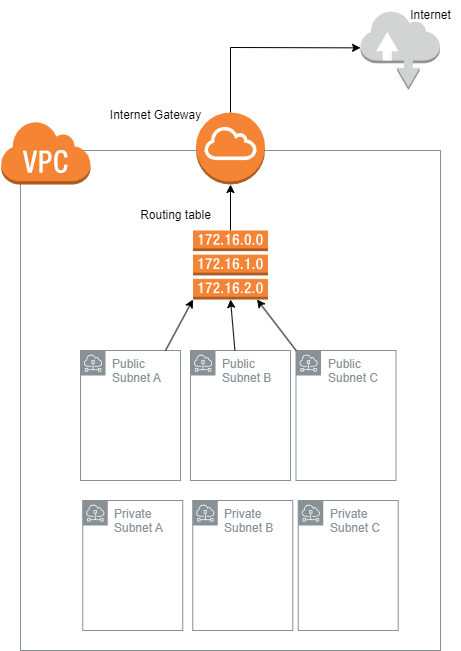
\includegraphics[width=1\columnwidth]{case_study/vpc_diagram} 
  \captionof{figure}{Infrastrutcture Architecture}
\end{center}\mbox{}\\
AWS is divided into regions, like us-east-1, eu-central-1, eu-south-1, etc.
For the purpose of our thesis eu-south-1 as a region has been chosen.
The servers of such a region are located in Milan.
Each region can have multiple availability zones, eu-south-1 has 3 different availability zones, and because of this we chose to create 3 couples of public/private subnets (A-A, B-B, C-C).
One couple on each availability zone.
The purpose of the availability zones is mainly for robustness.
If an availability zone becomes temporary unavailable, we can rely on the others to keep our services up.


\subsubsection{VPC}
The VPC is our "container" for all the other infrastructure resources.
We'll define within it the subnets, the internet gateway and the outing table.\\
The most important setting of our AWS EC2 VPC is the CIDR (Classless Inter-Domain Routing) block.
It represents the range of private IP addresses that the VPC can use to create and manage resources within the VPC.
\paragraph{CIDR}
The CIDR block is used to define the range of IP addresses that the VPC can use.
In our case the CIDR block is 10.136.0.0/24, which means that the VPC has access to all IP addresses from 10.136.0.0 to 10.136.0.255.
The 24 in the CIDR block is the prefix length, aka the subnet mask, that is used to identify the VPC.
The remaining 8 bits of the IP address will be used to identify the hosts in the VPC.\\
We'll assign a name as well to our VPC so that will be easier to recognize it when we'll inspect the AWS Management Console, that is the GUI version of the AWS CLI.

%val pvtSubnetsCidrs: List[String] = List("10.136.0.0/27", "10.136.0.32/27", "10.136.0.64/27")
%val pubSubnetsCidrs: List[String] = List("10.136.0.96/27", "10.136.0.128/27", "10.136.0.160/27")

\subsubsection{Subnet}
The subnets will require the ID of the VPC and the CIDR block that defines their IP scope.
For the subnets we'll use the following CIDR blocks:
\begin{itemize}
  \item Private Subnet A: 10.136.0.0/27
  \item Private Subnet B: 10.136.0.32/27
  \item Private Subnet C: 10.136.0.64/27
  \item Public Subnet A: 10.136.0.96/27
  \item Public Subnet B: 10.136.0.128/27
  \item Public Subnet C: 10.136.0.160/27
\end{itemize}
3 of the 8 bits left out for the hosts identification have been used to identify the subnets.
In fact we shall notice that now the subnet mask is not 24 anymore, but 27.
Hence, we are left with 5 bits to identify the hosts within each subnet, giving us 32 possible IPs.
From such IPs 2 are reserved for the network address and the broadcast address, so we have 30 possible IPs.
We won't discuss this topic any further since it isn't essential for the final objective of the thesis.\\
Moreover, we'll define also the availability zone for each subnet.


\subsubsection{InternetGateway}
The definition of the internet gateway is actually quite straight forward.
The mandatory parameter to assign is the ID of the VPC.

\subsubsection{RouteTable}
\label{sssec:routetable}
The definition of a route table is required in order to bind the public subnets to the internet gateway, so that they can send and receive data over the internet.\\
Here, along with the VPC ID, we assign the routes of such routing table.
In order to do this we have to provide a CIDR and a target resource to which the packet will be forwarded to, that can be a subnet or the internet gateway in our case.
The internet gateway is mapped with the CIDR block 0.0.0.0/0.
Obviously also the ID of the internet gateway is required in order to bind it to the routing table.\\
In a nutshell this means that every packet not directed to a host within the VPC will be routed to the internet gateway and then to the internet.\\
The association of the public subnets to the routing table will be achieved using the \textit{route table association} resource.
Such a resource will require us to provide the id of the subnet and the id of the routing table to establish a connection.
The private subnets will not be associated to such a routing table, since we want to keep them private.
Differently, without explicitly associating them to a given routing table, AWS will automatically associate them to a default routing table that, being not bound to an internet gateway, will keep them private.\\


\section{Typescript implementation of the case study}
\label{sec:typescript-impl}
The first version of the implementation of the previously defined architecture is written using the Typescript APIs of Pulumi.
The structure of the project, and this holds for the Java and Scala version as well, is trivial.
We have a simple \texttt{index.ts} file that defines the entry point for our typescript project, and it is just a couple of lines long:
\begin{lstlisting}[numbers=left, numberstyle=\tiny, numbersep=-5pt, stepnumber=1]
  import { VPC } from './VPC/VPC';

  const vpc = new MyVPC("Custom VPC");
\end{lstlisting}\mbox{}\\
The interesting part relies on the \texttt{MyVPC} class.
Such a class extends the \texttt{ComponentResource} class of Pulumi.
In our typescript implementation, we use the constructor of the user-defined \texttt{MyVPC} class to call all the class methods that are responsible for the creation of the resources.
But this is just mentioned since the interesting part of the code are the actual methods that are responsible for the creation of the resources.

\subsection{VPC resource creation}
The code to the VPC resource creation API of Pulumi is done in this method of the \texttt{MyVPC} class:
\begin{lstlisting}[numbers=left, numberstyle=\tiny, numbersep=-5pt, stepnumber=1]
  protected createVPC() {
    this.vpc = new Vpc("vpc\_res", {
      cidrBlock: "10.136.0.0/24",
      tags: {
        Name: "myVPC-typescript",
      },
    },
    {
      parent: this,
    });
  }
\end{lstlisting}\mbox{}\\
\texttt{vpc\_res} is the name that will be given by Pulumi at this resource once on the stack.
We can notice how the various parameters are given in a declarative style within the curly brackets.
Such a syntax is syntactic sugar for a Map definition.\\
At line 8 the parent of this resource is set.
With this specification, we are telling to the stack of Pulumi that the vpc resource \texttt{vpc\_res} that we are creating is a child resource of the VPC resource identified by the \texttt{MyVPC} class.

\subsection{Internet gateway creation}
To create the internet gateway resource we can use the following code:
\begin{lstlisting}[numbers=left, numberstyle=\tiny, numbersep=-5pt, stepnumber=1]
  protected createIGW(){
    this.gw = new InternetGateway("gw", {
      vpcId: this.vpc?.id,
      tags: {
          Name: "myIGW-typescript",
      },
    },
    {
      parent: this.vpc,
    });
  }
\end{lstlisting}\mbox{}\\
It is really simple since it requires just the ID of the VPC in which it has to be created and optionally a name and a parent for the Pulumi's stack representation.


\subsection{Subnets creation}
To create the private and the public subnets we require a more complex logic.
The function that has been used is \texttt{protected createAZsSubnets(isPvt: Boolean)}.
It is called twice, once with a true value to create the private subnets, and another one with false to instantiate the public ones (and connect them to the routing table bound with the internet gateway).\\
In the body of the function, first we want to get all the availability zones present in the AWS region we are working on.
To achieve this, we will use such a function \texttt{this.availableZones = aws.getAvailabilityZonesOutput()}.\\
Second, we want to create both a private and public subnet in each availability zone acquired with the aforementioned method.
The \texttt{pulumi.all} function, in combination with the \texttt{apply} function will help us in achieving such a goal.\\

\subsubsection{pulumi.all}
\label{sssec:pulumi-all}
\texttt{pulumi.all} is a utility function in Pulumi that allows you to combine multiple Outputs into a single Output that resolves to an array of the resolved values of each Output.
So if we consider the following code:
\begin{lstlisting}[numbers=left, numberstyle=\tiny, numbersep=-5pt, stepnumber=1]
  pulumi.all([this.availableZones.names, this.vpc!.id])
\end{lstlisting}\mbox{}\\
Such a call returns us an \texttt{Output<[string[], string]>}.
The array of strings is the list of the availability zones names, while the second string represents the ID of our VPC on AWS EC2.
Now we have a new Output type that is more suitable to create the subnets based on our VPC ID, because the function apply is letting us "open" an \texttt{Output} value and access its content.

\subsubsection{.apply}
Lets extend our code in this way:
\begin{lstlisting}[numbers=left, numberstyle=\tiny, numbersep=-5pt, stepnumber=1]
  pulumi.all([this.availableZones.names, this.vpc!.id]).apply(([azNames, vpcId]) => {
    // lambda's body to create the subnets here
  })
\end{lstlisting}\mbox{}\\
The apply function is letting us access \texttt{Output<[string[], string]>} and apply some logic on the inner values.\\

\paragraph{The apply's lambda}
\label{par:ts-lambda}
Now that we have the access to the list of availability zones and the VPC ID, we can iterate over the availability zones and create the subnets for our VPC.
Here is the complete code of the function:
\begin{lstlisting}[numbers=left, numberstyle=\tiny, numbersep=-5pt, stepnumber=1]
  protected createAZsSubnets(isPvt: Boolean) : Output<Subnet[]>{
    this.availableZones = aws.getAvailabilityZonesOutput()
    return pulumi.all([this.availableZones.names, this.vpc!.id]).apply(([azNames, vpcId]) => {
      let i = 0
      let listToPushInto: Subnet[] = Array<aws.ec2.Subnet>()
      azNames.forEach(azName => {
        let fullName = azName + (isPvt ? "-pvt" : "-pub") + "-subnet-typescript"
        listToPushInto.push(new Subnet(fullName, {
          vpcId: vpcId,
          availabilityZone: azName,
          cidrBlock: isPvt ? this.pvtSubnetsCidrs[i] : this.pubSubnetsCidrs[i],
          tags: {
            Name: fullName,
          },
        },{
          parent: this.vpc
        }));
        i++;
      });
      return listToPushInto
    });
  }
\end{lstlisting}\mbox{}\\
In the code we instantiate private or public public subnets basing on the \texttt{isPvt} passed in the \texttt{createAZsSubnets}.
We can notice that for the creation of a subnet we pass arguments such as \texttt{vpcId}, the availability zone name, the CIDR block, and a name (that is a tag) to better identify it on the stack.\\
Each newly created subnet is then pushed into the class field \texttt{this.prvSubNets} or \texttt{this.pubSubNets} (that are arrays of subnets), basing on the nature of the subnet.\\
The creation of a subnet requires us to provide both the availability zone name and the ID of the VPC.
Since these two pieces of information are contained in two separate \texttt{Output}s (\texttt{Output<String[]>} and \texttt{Output<String>} respectively) we must first use the \texttt{pulumi.all} to wrap them in a single \texttt{Output<String[], String>}.
This due to the fact that \texttt{.apply} can accept a single \texttt{Output<A>}, for any \texttt{A} type, value as input and not a pair.
Then, we can use the \texttt{.apply} to unbox from the \texttt{Output<String[], String>} its inner value.
Now that we have both the pieces of information out of the context value, we can use them to create the subnets.\\
%The \texttt{this.pubSubNets} will be used by the \texttt{this.attachRouteTableToPubSubnets()} function to bind the public subnets to the internet gateway through the routing table.\\
%The crucial point here is that in order to bind the public subnets to the routing table, we must call \texttt{this.attachRouteTableToPubSubnets()} as the last step in our \texttt{pulumi.all} function call.
%This ensures that we have all the necessary subnets to make the binding, since the call will be done at the completion of the creation of the subnets.
We can notice that the \texttt{.apply} function is, at the end of its lambda function, returning a list of the created subnets.
Such a return is also the return of the function and is indeed of the \texttt{Output<Subnet[]>} type.

\subsection{Routing table creation}
This is the code to create the routing table resource:
\begin{lstlisting}[numbers=left, numberstyle=\tiny, numbersep=-5pt, stepnumber=1]
  protected createRouteTable() {
    this.routeTable = new RouteTable("example", {
      vpcId: this.vpc!.id,
      routes: [
          {
              cidrBlock: "0.0.0.0/0",
              gatewayId: this.gw!.id,
          },
      ],
      tags: {
          Name: "myRouteTable-typescript",
      },
  },
  {
    parent: this.vpc,
  });
  }
\end{lstlisting}\mbox{}\\
On top of the classic VPC ID we are assigning here the routes.
As we mentioned before in the \hyperref[sssec:routetable]{Routetable} paragraph, we are defining the route with CIDR 0.0.0.0/0 to redirect all the packets coming from the public subnets, and not having as destination an IP internal at our VPC, to the internet gateway.\\
We are also giving a name to the routing table and assigning its parent.


\subsection{Attaching the public subnets to the internet gateway}
As we mentioned previously, we use the \texttt{this.attachRouteTableToPubSubnets()} function to attach the public subnets to the internet gateway.
Here is the code of the function:
\begin{lstlisting}[numbers=left, numberstyle=\tiny, numbersep=-5pt, stepnumber=1]
  protected attachRouteTableToPubSubnets(){
    let i = 0
    this.pubSubNets.apply(subNets => {
      subNets.forEach(sn => {
        new aws.ec2.RouteTableAssociation(`${i}-routeTableAssociation-typescript`, {
          subnetId: sn.id,
          routeTableId: this.routeTable!.id,
        },
        {
          parent: this.vpc
        });
        i++
      })
    });
  }
\end{lstlisting}\mbox{}\\
Here we used once more, as for the subnets creation, a combination of \texttt{.apply} and a foreach to iterate over all the extracted subnets (\texttt{.foreach}) from the Output context (\texttt{.apply}).\\
Inside the \texttt{foreach}'s lambda we are defining a new \texttt{RouteTableAssociation} AWS EC2 resource that requires just the id of the subnet and the id of the routing table to which we want to attach the subnet to.

\section{Creating the resources with Pulumi}
After having seen all the code to create the resources, we'll see what the Pulumi command \texttt{pulumi up} will do.
The command checks if all the resources that we want to create have valid parameters and there are not circular dependencies among the resources on their creation.
If everything is nice and neat, it will shows us the preview of the changes that we are about to get:
\begin{center}
  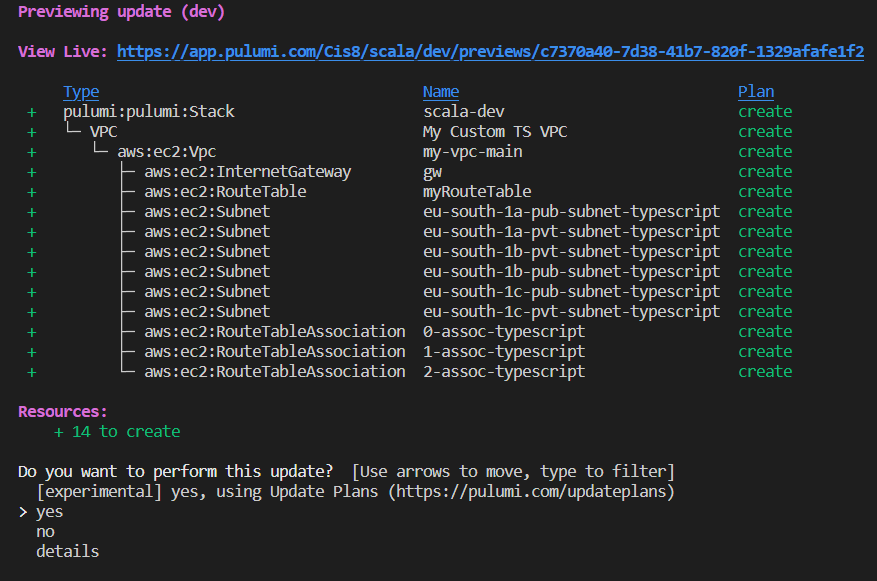
\includegraphics[width=1\columnwidth]{case_study/pulumi_up_1} 
  \captionof{figure}{pulumi up preview}
\end{center}\mbox{}\\

If we press yes this is the output:
\begin{center}
  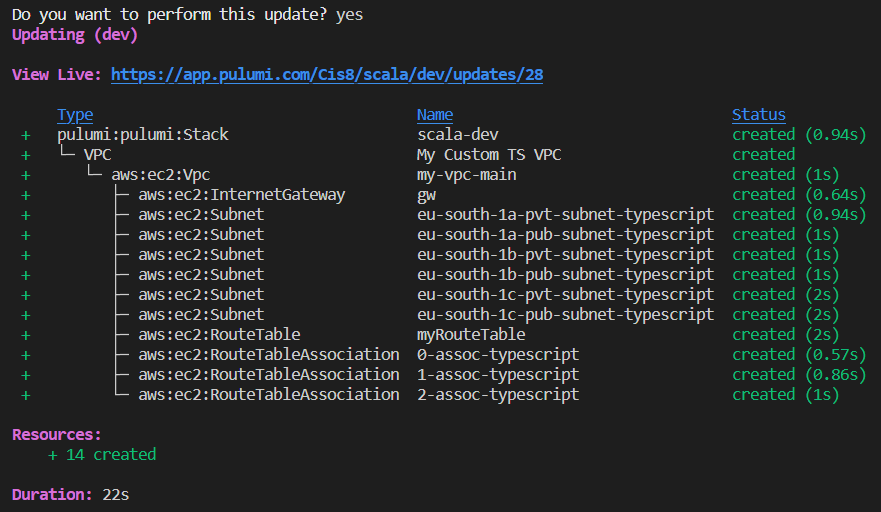
\includegraphics[width=1\columnwidth]{case_study/pulumi_up_2} 
  \captionof{figure}{pulumi up confirmed}
\end{center}\mbox{}\\
We can notice how the resources created are nested into each other thanks to the parent option that we used.
This is helping us in keeping our resources on the stuck nicely ordered and tied up.\\

\section{Destroying the resources with Pulumi}
Now lets use the \texttt{pulumi destroy} command to destroy the resources on our Pulumi's stack.
The preview of the changes that we are about to get look like this:
\begin{center}
  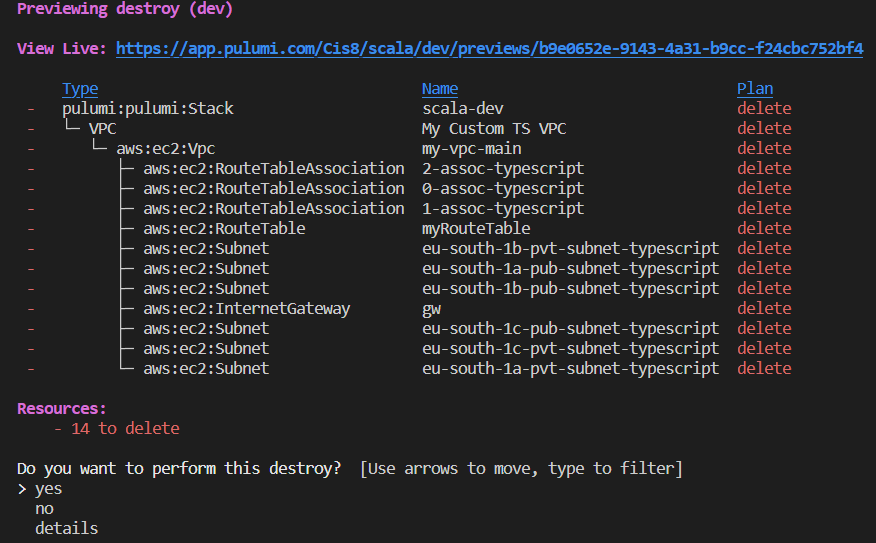
\includegraphics[width=1\columnwidth]{case_study/pulumi_destroy_1} 
  \captionof{figure}{pulumi destroy preview}
\end{center}\mbox{}\\

If we confirm the changes this is the result:
\begin{center}
  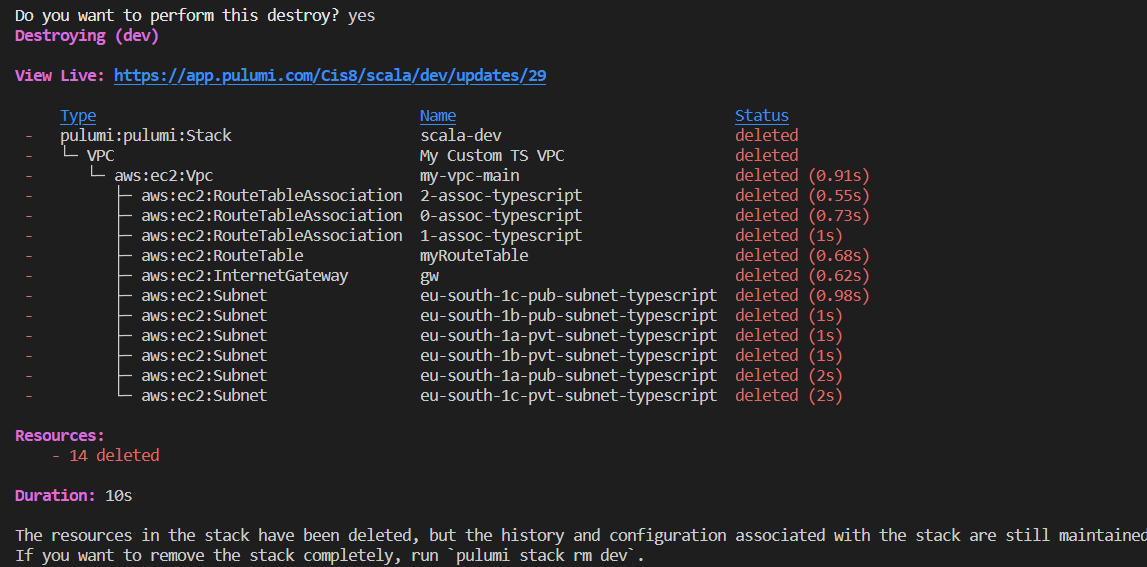
\includegraphics[width=1\columnwidth]{case_study/pulumi_destroy_2} 
  \captionof{figure}{pulumi destroy confirmed}
\end{center}\mbox{}\\

%\section{Java implementation of the case study}

\section{My Scala implementation of the case study}
Since Scala is not supported by Pulumi, I had to implement it on my own.
The Pulumi team is clear on the official way to add the support of a new language for Pulumi, and the procedure is long and laborious, too laborious for a master thesis.
The full procedure can be found on \href{https://github.com/pulumi/pulumi/wiki/New-Language-Bring-up}{New Language Bring Up}.\\
The idea behind the adopted solution is to exploit the compatibility of Scala with the Java libraries to write custom syntactic sugar.
Such syntactic sugar will be based on the Pulumi Java's APIs and will provide to the user cool constructs to write readable and expressive code to interact with Pulumi.\\
The steps of the work done have been the followings:
\begin{enumerate}
  \item manually write the \textit{sugarized} functions to create the Pulumi resources using Scala
  \item use such functions to recreate the Stack obtained with the typescript solution shown before in the \hyperref[sec:typescript-impl]{Typescript implementation of the case study} section
  \item create an automatic code generator for our syntactic sugar functions, so that we can quickly create a library for Scala's Pulumi APIs
  \item try to recreate the stack with the automatically generated code
\end{enumerate}
Obviously, the third step is quite wide, and if fact with my work I had the time to generate only the functions for a part of the Java's Pulumi APIs for the AWS EC2 module.\\
Now the just defined steps will more accurately presented.

\subsection{Structure of the Java APIs for the constructors of the resources in Pulumi}
To understand the syntactic sugar functions that I defined, let's first consider the general structure of the Java APIs for the constructors of the resources.\\
The constructor of a resource, in general accepts a name and an instance of the corresponding \texttt{Args} class of the resource we are creating.
Lets consider for example the Vpc resource.
In Java, to instantiate such a resource we'd call:
\begin{lstlisting}[numbers=left, numberstyle=\tiny, numbersep=-5pt, stepnumber=1]
  protected Vpc vpc = new Vpc("my-vpc-java", VpcArgs.builder()
    .cidrBlock("10.136.0.0/24")
    .tags(Map.of("Name", "main"))
    .build(),
          CustomResourceOptions.builder()
                  .parent(this)
                  .build());
\end{lstlisting}\mbox{}\\
We can (hardly) see that along with the name to be assigned to the vpc "my-vpc-java", a VpcArgs builder and a CustomResourceOptions builder are passed by.
These builders will create an instance of the respective classes that will be used to set respectively the parameters and the parent of the Vpc resource.
So, for our case study we need to consider: the name to be assigned at the created resource on the Pulumi stack, the builder of the respective \texttt{Args} class of the resource, and the \texttt{CustomResourceOptions} builder.


\subsection{Syntactic sugar usage}
\label{ssec:syn-sug-usage}
Our syntactic sugar is split in 2 categories of functions.
The first is about the functions that represent the constructors of the resources.
The second is for the methods available within the builders of the \texttt{Args} classes and for the CustomResourceOptions builder functions.
The idea to create a resource is to call the \textit{sugarized} function that represent the constructor of that resource, and and then call the Builder methods to assign the various parameters to the resource.

\subsubsection{Vpc creation}
\label{sssec:vpc-creation-scala}
This is how a Vpc resource can be created with my syntactic sugar:
\begin{lstlisting}[numbers=left, numberstyle=\tiny, numbersep=-5pt, stepnumber=1]
  val myVpc = vpc("scala-main") ({
    cidrBlock("10.136.0.0/24")
    tags("Name" -> "myVpcScala")
  },{
    parent(this)
  })
\end{lstlisting}\mbox{}\\
At line 1, the \texttt{vpc} function is the actual \textit{sugarized} function for the VPC resource constructor.
In fact we can notice that we have a curried function.
The first parentheses is taking the parameter for the resource name on the Pulumi stack, while the second one is containing two lambdas (defined by the curly brackets).
These lambdas are respectively used to call all the builder methods of the \texttt{VcpArgs} class and the ones for the \texttt{CustomResourceOptions}.\\
We can notice that we didn't explicitly defined an instance of the builders of such classes.
We will soon see how we achieved such a syntactic sugar trick.\\
The \texttt{cidrBlock} and the \texttt{tags} methods are the generated methods for builder of the \texttt{VpcArgs} class.\\ 
The \texttt{parent} method instead is the generated method for the builder of the \texttt{CustomResourceOptions} class.\\
Moreover, we can also notice that inside tags, that expects a \texttt{Map[String, String]} type, the instantiation of a \texttt{Map[String, String]} containing a single elements isn't required.
This other trick will be explained later as well.

\subsubsection{Internet gateway creation}
Much similar to the VPC resource, we have this code for the internet gateway creation:
\begin{lstlisting}[numbers=left, numberstyle=\tiny, numbersep=-5pt, stepnumber=1]
  val myIGW = internetGateway("gw") ({
    vpcId(myVpc.getId())
    tags("Name" -> "myIGWScala")
  },{
    parent(myVpc)
  })
\end{lstlisting}\mbox{}\\
The code won't be commented since is analogous to the VPC case.

\subsubsection{Routing table creation}
\label{sssec:routetable-creation-scala}
The code to create a routing table:
\begin{lstlisting}[numbers=left, numberstyle=\tiny, numbersep=-5pt, stepnumber=1]
  val myRouteTable = routeTable("myRouteTable") ({
    vpcId(myVpc.getId())
    routes(
      routeTableRouteArgs(){
        cidrBlock("0.0.0.0/0")
        gatewayId(myIGW.getId())
      })
    tags("Name" -> "myRouteTableScala")
  },{
    parent(myVpc)
  })
\end{lstlisting}\mbox{}\\
The only thing that is worth to mention here is that the \texttt{routes} function, at line 3, expects a \texttt{List[RouteTableRouteArgs]}, but we are providing only a \texttt{RouteTableRouteArgs}.
As for the case of the \texttt{Map[String, String]} with the parent method mentioned above, the same trick has been used to provide syntactic sugar that lifts us from the need of instantiate a singleton \texttt{List[RouteTableRouteArgs]} manually.

\subsubsection{Subnets creation}
\label{sssec:subnets-creation}
Much different from the other resources is the function to create the subnets:
\begin{lstlisting}[numbers=left, numberstyle=\tiny, numbersep=-5pt, stepnumber=1,linewidth=420pt]
  def createAzSubnets(isPvt: Boolean) =
    availabilityZonesNames().map((az: GetAvailabilityZonesResult) =>
      for
        (name, cidr) <- az.names().zip(if isPvt then pvtSubnetsCidrs else pubSubnetsCidrs)
      yield
        val fullName = name + "-" + (if isPvt then "pvt" else "pub") + "-subnet-scala"
        subnet(fullName) ({
          vpcId(myVpc.getId())
          availabilityZone(name)
          cidrBlock(cidr)
          tags("Name" -> fullName)
        },{
          parent(myVpc)
        })
    )
\end{lstlisting}\mbox{}\\
We can notice here how we had the possibility to use the \texttt{map} function on \texttt{availabilityZonesNames()}.
\texttt{availabilityZonesNames()} returns a \texttt{Output[GetAvailabilityZonesResult]} value, that isn't directly accessible from the \texttt{map} function.
To achieve such a result we made a monad out of the \texttt{Output} type, so that map can be applied on the inner value of the \texttt{Output} context.
We'll see better how is the actual implementation of the monad soon.\\
The for yield construct here is iterating over a zipped list made out of the availability zones names and the CIDR blocks for the respective kind of subnet to create (private or public, based on the input parameter isPvt).
The for yield, for each tuple \texttt{(name, cidr)} will create a \texttt{Subnet} value and will return a \texttt{Subnet[]} as output.
Now, the for is still inside the lambda of the \texttt{availabilityZonesNames().map} function.
Consider the fact that \texttt{map} takes an \texttt{Output[A]} and returns an \texttt{Output[B]}, where \texttt{A = GetAvailabilityZonesResult} and \texttt{B = Output[Iterable[Subnet]]}.
This is different from the typescript implementation in the \hyperref[par:ts-lambda]{Apply's lambda} paragraph, where the function that creates the subnets returns a plain \texttt{Subnet[]}.\\
We will make further considerations about such a difference in the \hyperref[cap:comparisons]{Comparison between the languages for Pulumi and the advantages of Scala} chapter.\\

\subsubsection{Attaching the subnets to the routing table}
\begin{lstlisting}[numbers=left, numberstyle=\tiny, numbersep=-5pt, stepnumber=1]
  def attachRouteTableToPubSubnets(): Output[Iterable[RouteTableAssociation]] =
    pubSubnets.map((subnets: Iterable[Subnet]) =>
        for
          (ps, idx) <- subnets.zipWithIndex
        yield
          routeTableAssociation(idx + "-assoc-scala") ({
            subnetId(ps.getId())
            routeTableId(myRouteTable.getId())
          }, {
            parent(myVpc)
          })
      )
\end{lstlisting}\mbox{}\\
Similarly to the subnet creation function, also here we use map to "unbox" an \texttt{Output[Iterable[Subnet]]} value, to apply some logic on the inner value and then return a \texttt{Output[Iterable[RouteTableAssociation]]} value as result.
Since the logic is analogous we won't comment this code further, but the fact we're having these two functions that both take an Output[A] as input and return an Output[B] will be a key point for our observations in the \hyperref[cap:comparisons]{Comparison between the languages for Pulumi and the advantages of Scala} chapter.

\subsubsection{Resources creation with pulumi up}
\label{sssec:res-cre-ts}
Now lets make sure that the stack created with \texttt{pulumi up} is the same of the one created with the typescript implementation.
From this image we can see that they are equivalent to the ones shown in \hyperref[sssec:res-cre-ts]{Resources creation with pulumi up in Typescript}:
\begin{center}
  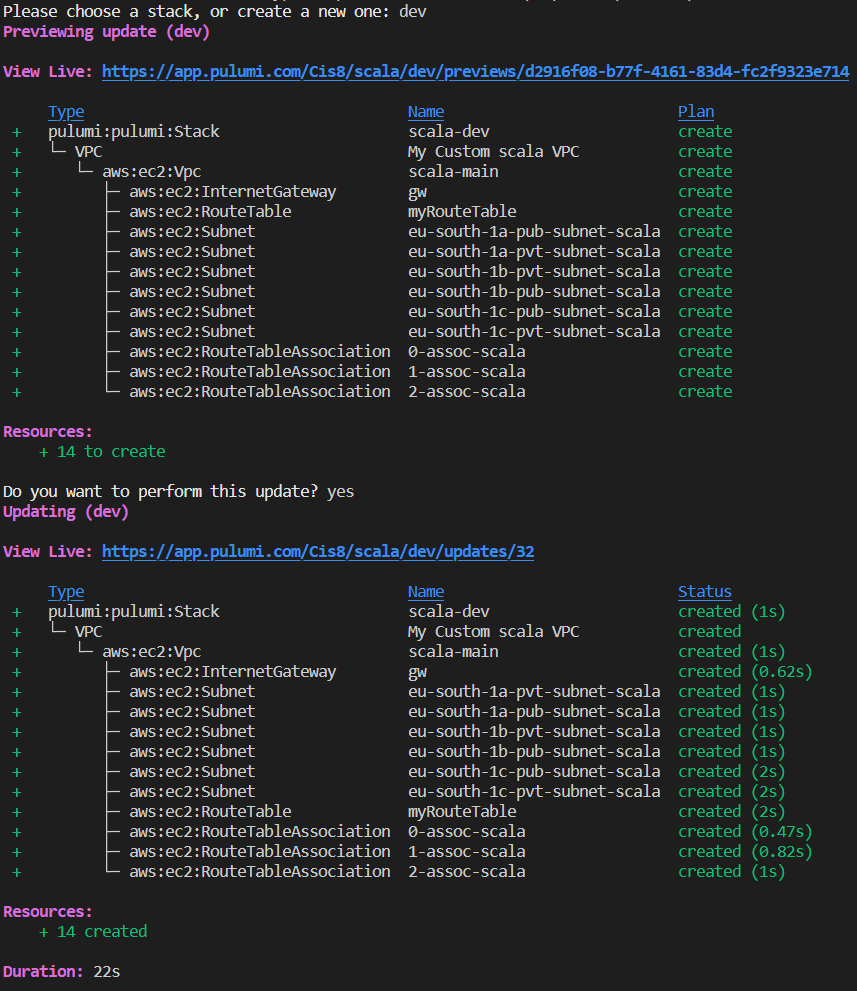
\includegraphics[width=1\columnwidth]{case_study/pulumi_up_scala_result} 
  \captionof{figure}{pulumi up result with the scala implementation}
\end{center}\mbox{}\\

\subsection{Syntactic sugar for the constructors of the resources}
All the methods that we just used for creating the Pulumi resources in Scala (\texttt{vpc, internetGateway}, ecc.), behind the scenes are implemented following a common pattern.
Consider the vpc function of the syntactic sugar defined inside the "PulumiUtilFunctionsForScala.scala" file:
\begin{lstlisting}[numbers=left, numberstyle=\tiny, numbersep=-5pt, stepnumber=1]
  def vpc(param: String)
         (init: VpcArgs.Builder ?=> Unit,
          initOpt: (CustomResourceOptions.Builder ?=> Unit) = baseOpts): Vpc =
	  given b: VpcArgs.Builder= VpcArgs.builder()
	  init
	  given bo: CustomResourceOptions.Builder = CustomResourceOptions.builder()
	  initOpt
	  new Vpc(param, b.build(), bo.build())
\end{lstlisting}\mbox{}\\
Lets analyze the function by steps.
First of all we can see that the function declaration is curried, we have 2 parentheses with different input parameters.\\
The first parentheses take simply a string parameter, that is used to set the name of the \texttt{Vpc} resource on the Pulumi stack.\\
The second parentheses are taking two lambdas as parameters: a \texttt{VcpArgs.Builder ?=> Unit}  and a \texttt{CustomResourceOptions.Builder ?=> Unit}, with default parameter baseOpts, that we'll see in a moment what is.\\
In Scala, a lambda that takes an Int and returns a String has this type notation: \texttt{Int => String}, so does that '\texttt{?}' in front of the '\texttt{=>}' mean?\\
Such '\texttt{?=>}' is denoting a context function, that is a function with (only) context parameters.
In the \hyperref[par:given-using]{Given and using keywords} paragraph we introduced the \texttt{using} keyword.
Such '\texttt{?}' is quite analogous to a \texttt{using} keyword used to mark an function's input parameter as a context parameter.
This is, in part, what let us call the builder methods like \texttt{cidrBlock("10.136.0.0/24")} and \texttt{tags("Name" -> "myVpcScala")} (as shown in the code shown in the \hyperref[sssec:vpc-creation-scala]{Vpc creation in Scala} paragraph)
without having to call them on a specific builder instance.
We will get the whole picture of this trick when we'll talk about the syntactic sugar for the builder methods in the \hyperref[ssec:syn-sug-builders]{Syntactic sugar for the builders' methods} paragraph.

\subsubsection{Correspondence between the input parameters and the user defined code used to create the VPC}
To have a better idea to what these parameters refer in our VCP creation case, consider this image:
\begin{center}
  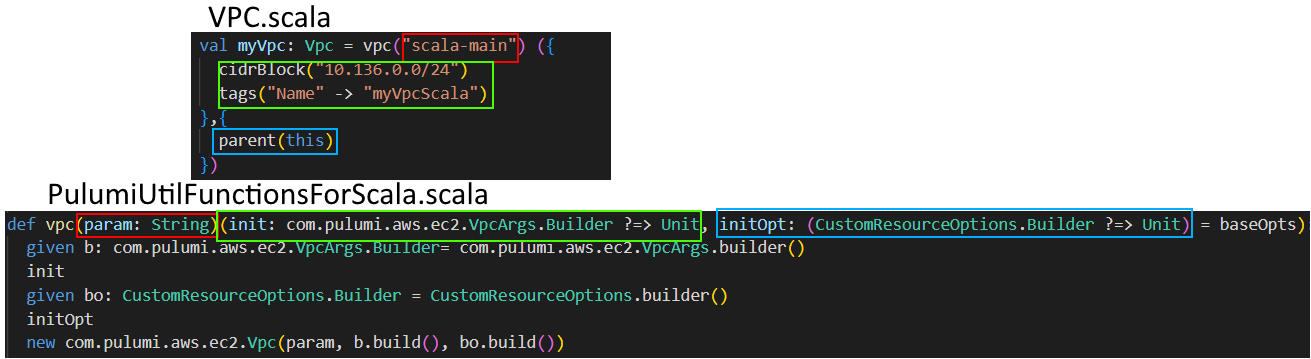
\includegraphics[width=1.3\columnwidth]{case_study/vpc_params_boxes} 
  \captionof{figure}{Parameters correspondence}
\end{center}\mbox{}\\
The red box represents the name for our VPC resource on the Pulumi stack.\\
The green one, with the curly brackets, is the lambda that takes a \textit{given} \texttt{VpcArgs.Builder} as an implicit parameter from the context.
In fact we are not providing any explicitly.
The \texttt{given b} defined in the first line of the body of the \texttt{vpc} function is the instantiation of a \textit{given} instance of such a builder, that will be automatically injected by the compiler in the \texttt{init} lambda represented by the green box.\\
Analogous is the concept for the blue box.\\

\subsubsection{Vpc construction}
Now that we understood what are the input parameters of our \texttt{vpc} function and to what do they correspond in the resource creation shown in the \hyperref[ssec:syn-sug-usage]{Syntactic sugar usage} section, we can see how the actual creation of the resource is made.
After having executed the \texttt{init} and \texttt{initOpt} lambdas, that behind the scenes will set the parameters of the respective \textit{given} builders, we can create the resource using the constructor offered by the Pulumi Java APIs.
\texttt{new Vpc(param, b.build(), bo.build())} is a direct call to such libraries, and will create actually create the \texttt{VPC}.

\subsubsection{The baseOpts function}
The \texttt{baseOpts} function that we mentioned before as a default lambda for our \texttt{vpc} function is the following:
\begin{lstlisting}[numbers=left, numberstyle=\tiny, numbersep=-5pt, stepnumber=1]
  def baseOpts(using o: CustomResourceOptions.Builder) : Unit = {}
\end{lstlisting}\mbox{}\\
In practice, is an vacuous lambda that does nothing on the \texttt{CustomResourceOptions} builder.
The question here is: \textit{why do we need such a default function?}
To answer the question let's consider one more time the code to create a VPC with out syntactic sugar:
\begin{lstlisting}[numbers=left, numberstyle=\tiny, numbersep=-5pt, stepnumber=1]
  val myVpc: Vpc = vpc("scala-main") ({
    cidrBlock("10.136.0.0/24")
    tags("Name" -> "myVpcScala")
  },{
    parent(this)
  })
\end{lstlisting}\mbox{}\\
We can see that we passed both the lambdas for the \texttt{VpcArgs} builder and for the \texttt{CustomResourceOptions} builder, but what if we want to simply use the \texttt{VpcArgs} builder and not set the parent?
We can do the following:
\begin{lstlisting}[numbers=left, numberstyle=\tiny, numbersep=-5pt, stepnumber=1]
  val myVpc: Vpc = vpc("scala-main") {
    cidrBlock("10.136.0.0/24")
    tags("Name" -> "myVpcScala")
  }
\end{lstlisting}\mbox{}\\
This code compiles, and we can notice that we even got rid of the parentheses around the two groups of curly brackets for the lambdas.
If this compiles is only thanks to the default parameter that is automatically injected in by the compiler, as we didn't give an explicit one.\\
Another question now might arise: \textit{why didn't we change the signature of the function in the following way?}
\begin{lstlisting}[numbers=left, numberstyle=\tiny, numbersep=-5pt, stepnumber=1]
  def vpc(param: String)(using initOpt: (CustomResourceOptions.Builder ?=> Unit), init: VpcArgs.Builder ?=> Unit) : ecc.
\end{lstlisting}\mbox{}\\
Here we have set the \texttt{initOpt} as an implicit parameter with the \texttt{using} keyword.
The main problems that we face with this solution are mainly 2: we have to swap the order of the parameters and we will be forced to use the \textit{using} keyword to explicitly pass a custom lambda for the \texttt{CustomResourceOptions} builder.\\
The first problem leads to a sort of awkwardness while defining the VPC resource, since we have to define first the parent and then the actual parameters of the VPC resource.\\
The second problem is requiring us to write \texttt{using} every time we want to pass an explicit and custom lambda that sets some parameters of the \texttt{CustomResourceOptions} builder, that is annoying.\\
These problems are due to the functioning of the Scala language.
An implicit parameter must come before all the explicit parameters and when trying to use an explicit parameter in place of an implicit one we must use the \texttt{using} keyword.
So, the original solution with the default parameter is the best one since it doesn't require us to swap the order of the parameters and we are totally free to choose whether to pass or not the explicit lambda for the \texttt{CustomResourceOptions} builder without worsening our syntactic sugar.


\subsection{Syntactic sugar for the builders' methods}
\label{ssec:syn-sug-builders}
What we have shown up to now is not enough to have our syntactic sugar working, we are missing a subtle point to get the work done.
Lets pay attention to how the \texttt{VpcArgs.Builder} parameters are set inside the vpc function call.
To be precise we are referring to these methods:
\begin{center}
  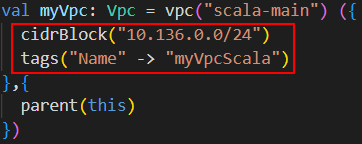
\includegraphics[width=0.5\columnwidth]{case_study/vpc_b_methods} 
  \captionof{figure}{vpc methods}
\end{center}\mbox{}\\
Once such a lambda will be invoked inside the vpc function itself, these methods will be executed, but on which builder?\\
We already mentioned the fact that inside the vpc function a context instance of the VpcArgs.Builder is initialized and the \texttt{init} lambda is able to use it as input parameter thanks to the '\texttt{?=>}' operator we have seen.
But how can the actual \texttt{cidrBlock} and \texttt{tags} methods know on which builder they are being invoked?\\
Without surprise, those methods take the \texttt{VpcArgs.Builder} builder as an implicit parameter with the \texttt{using} keyword.\\
This is the signature for the \texttt{cidrBlock} method in the syntactic sugar file named "PulumiBuilderUtilFunctionsForScala.scala":
\begin{lstlisting}[numbers=left, numberstyle=\tiny, numbersep=-5pt, stepnumber=1, linewidth=420pt]
  def cidrBlock(param: String | Output[String]) (using b: cidrBlockOwners): Unit
\end{lstlisting}\mbox{}\\
We can notice that we have once more a curried function.
Anyway, from how we have seen before, the \texttt{cidrBlock} (and analogously for all the other builder methods) is called with just a single set of parentheses.
This is due to the fact that the second parentheses here are taking an implicit parameter, properly marked with the \texttt{using} keyword.\\
The \texttt{param} parameter is, as we have seen in the \hyperref[sssec:union]{Union type} paragraph, a union type.
The \texttt{String | Output[String]} type is defined so since the Pulumi Java APIs for the builders' methods accept bot a String and an Output[String].
Actually, in the Java implementation an overloading of methods is given since the union type of Scala is not available.\\
The second parentheses are taking an implicit parameter \texttt{b} of the type \texttt{cidrBlockOwners}, that is defined as follows:
\begin{lstlisting}[numbers=left, numberstyle=\tiny, numbersep=-5pt, stepnumber=1, linewidth=420pt]
  type cidrBlockOwners = RouteTableRouteArgs.Builder | SubnetArgs.Builder | VpcArgs.Builder
\end{lstlisting}\mbox{}\\
This is a user defined type that I defined to match the builders of all the \text{Args} classes that are interested in having such a parameter to assign on their builder instance.
In fact in the Java APIs of Pulumi we have many different \texttt{Args} classes' builders that want to assign the same parameter (aka. \texttt{cidrBlock}) to their own builder.
I remind that in the AWS EC2 module there are much more builders of the \texttt{Args} classes that define a cidrBlock method, but my syntactic sugar has created the methods for only the classes that I used in the case study.
This choice has been made also for simplicity in presenting the work done, otherwise the \texttt{cidrBlockOwners} type would have been featuring many tens of types.
The fact we used a union type to define this function has two main motivations.
The first is a Scala language constraint that we came across.
Lets say that we wanted to define a function to assign the CIDR block working exclusively for \texttt{VpcArgs.Builder} class.
A definition of such a function would look like:
\begin{lstlisting}[numbers=left, numberstyle=\tiny, numbersep=-5pt, stepnumber=1, linewidth=420pt]
  def cidrBlock(param: String | Output[String]) (using b: VpcArgs.Builder): Unit =
      param match
        case x: String => builder.cidrBlock(x)
        case x: Output[String] => builder.cidrBlock(x)
\end{lstlisting}\mbox{}\\
And now lets define another function that is working for the \texttt{RouteTableRouteArgs.Builder}:
\begin{lstlisting}[numbers=left, numberstyle=\tiny, numbersep=-5pt, stepnumber=1, linewidth=420pt]
  def cidrBlock(param: String | Output[String]) (using b: RouteTableRouteArgs.Builder): Unit =
      param match
        case x: String => builder.cidrBlock(x)
        case x: Output[String] => builder.cidrBlock(x)
\end{lstlisting}\mbox{}\\
First, we can notice that they are actually the same, except for the signature , but such a solution is not going to compile if we try to call the method \texttt{cidrBlock("10.136.0.0/24")} here:
\begin{lstlisting}[numbers=left, numberstyle=\tiny, numbersep=-5pt, stepnumber=1, linewidth=420pt]
  val myVpc: Vpc = vpc("scala-main") ({
    cidrBlock("10.136.0.0/24") \\ ERROR
    tags("Name" -> "myVpcScala")
  },{
    parent(this)
  })
\end{lstlisting}\mbox{}\\
The compiler will tell us that an ambiguous function call is present at the line 2 of this block of code.
This is due to the fact that the functions we defined are curried and their type is \texttt{(String | Output[String]) => (VpcArgs.Builder => Unit)} and \texttt{(String | Output[String]) => (RouteTableRouteArgs.Builder => Unit)} respectively.
When we call \texttt{cidrBlock("10.136.0.0/24")} on the line 2 of the code showed above, we are partially applying the curried function and so the compiler doesn't know which function we are trying to call, since it can't infer the exact function call basing only on a different return type (that is the only difference in the two functions).\\
The second reason is that our \textit{all-in-one} solution is reducing the size of the generated \textit{sugarized} code, since we have just one single method instead of having as many as the builders of the \texttt{Args} classes that require that methods are.\\

Now we are ready to present the entire \texttt{cidrBlock} method:
\begin{lstlisting}[numbers=left, numberstyle=\tiny, numbersep=-5pt, stepnumber=1, linewidth=420pt]
  def cidrBlock(param: String | Output[String]) (using b: cidrBlockOwners): Unit =
    b match
      case builder: RouteTableRouteArgs.Builder =>
        param match
          case x: String => builder.cidrBlock(x)
          case x: Output[String] => builder.cidrBlock(x)
      case builder: SubnetArgs.Builder =>
        param match
          case x: String => builder.cidrBlock(x)
          case x: Output[String] => builder.cidrBlock(x)
      case builder: VpcArgs.Builder =>
        param match
          case x: String => builder.cidrBlock(x)
          case x: Output[String] => builder.cidrBlock(x)
\end{lstlisting}\mbox{}\\
The body of the function is quite simple in its functioning.
It uses the pattern matching to match the correct builder type and then uses pattern matching once more to match the \texttt{param} parameter to a \texttt{String} or an \texttt{Ouput[String]}.
Finally it calls the Java API of Pulumi to set the cidrBlock parameter on the builder instance b.\\
The fact we have duplicated code here is inevitable.
This is the only solution since if we try to split the duplicated code into an helper function, we would fall again in the ambiguous call error presented above.
But since this is automatically generated code, it is not a real problem to have some duplicated code.\\

To have the final picture of all the functioning lets consider this image:
\begin{center}
  \hspace*{-3cm}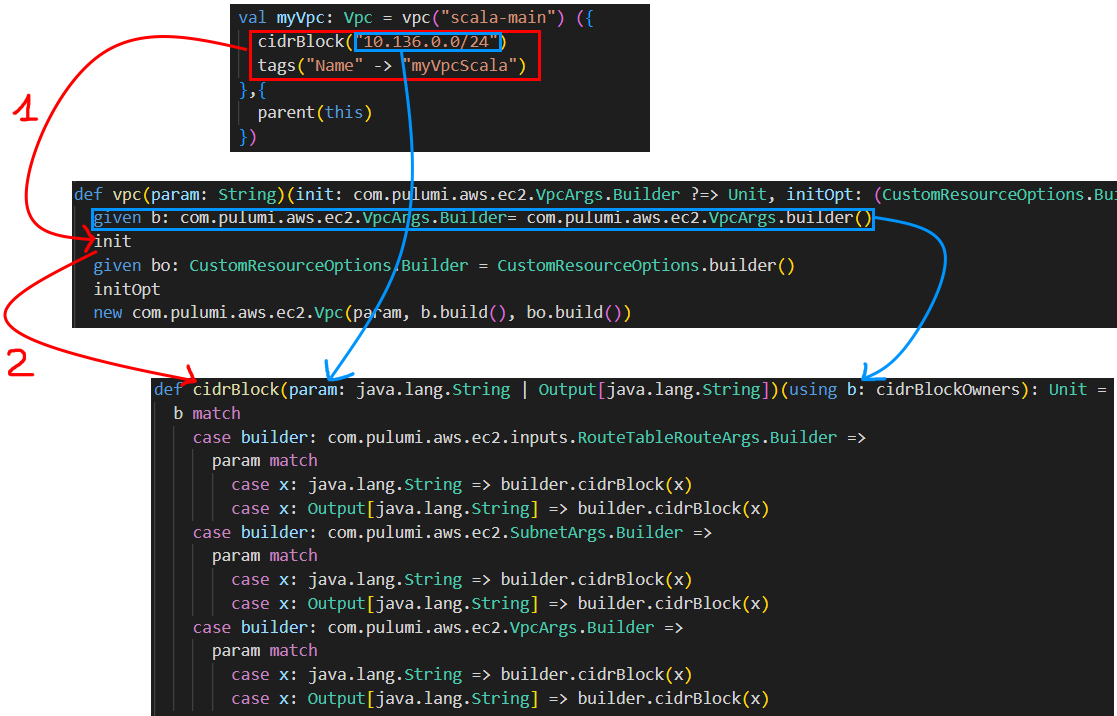
\includegraphics[width=1.4\columnwidth]{case_study/syn-sug-flow} 
  \captionof{figure}{Function calls flow and parameters passing}
\end{center}\mbox{}\\
We can see how the lambda with the calls to our defined methods \texttt{cidrBlock} and \texttt{tags} is passed as the \text{init} parameter of the \textit{sugarized} \texttt{vpc} function.
Inside the \texttt{vpc} function we execute that lambda and so, the \texttt{cidrBlock} method is invoked.\\
In blue we can see from where the parameters of the \texttt{cidrBlock} method are coming from.
The \texttt{String} representing the CIDR block is coming directly from the explicit parameter that we passed,
while the \texttt{VpcArgs} builder is implicitly injected from the compiler since a \textit{given} instance is defined inside the vpc function and the \texttt{b} parameter of the \texttt{cidrBlock} method is marked with \texttt{using}.

\subsubsection{Implicit conversion functions}
\label{sssec:implicit-converion-functions}
On top of this, to boost our syntactic sugar I defined also two extra functions: \texttt{tupleToMap} and \texttt{elemToList}.
The purpose of this functions is to achieve the tricks that I mentioned previously (in the \hyperref[sssec:vpc-creation-scala]{Vpc creation in Scala} and in the the \hyperref[sssec:routetable-creation-scala]{Routetable creation in Scala}) about not needing to explicitly instantiate a singleton Map and a singleton List while passing a single argument to the \texttt{tags} or the \texttt{routes} methods.
The \texttt{tupleToMap} function is implemented like this:
\begin{lstlisting}[numbers=left, numberstyle=\tiny, numbersep=-5pt, stepnumber=1, linewidth=420pt]
  given tupleToMap[A, B]: Conversion[(A, B), Map[A, B]] =
	  (tuple: (A, B)) => Map(tuple)
\end{lstlisting}\mbox{}\\
We can notice that the function that converts our tuple into a singleton Map is based on the Converion class of Scala.
When a suitable argument for the conversion of type (A, B) is found in the code, and a Map[A, B] type is expected, then the compiler will apply the conversion to that type.
This is exactly what happens with our tuple as single parameter passed to the \texttt{tags} method.\\
And the \texttt{elemToList} function is defined in this way instead:
\begin{lstlisting}[numbers=left, numberstyle=\tiny, numbersep=-5pt, stepnumber=1, linewidth=420pt]
  given elemToList[A <: ResourceArgs]: Conversion[A, List[A]] =
	  (elem: A) => List(elem)
\end{lstlisting}\mbox{}\\
The functioning is analogous to \texttt{tupleToMap}, but here we added the extra constraint that A must be a subtype of the \texttt{ResourceArgs} type.
This will prevent undesired too generic conversions that could create problems in the compilation of our program.

\subsection{Functor and Monad implementation for the Output type}
After having introduced the concept of functor and monad in the \hyperref[sssec:functors-monads]{Functor and monads} section, it is here show how the implementation of the monad for the \texttt{Ouput} type has been achieved.\\
Since a monad is also a functor, lets see how \texttt{Functor[Output]} has been implemented.

\subsubsection{Functor implementation}
First a \texttt{Functor} trait has been defined:
\begin{lstlisting}[numbers=left, numberstyle=\tiny, numbersep=-5pt, stepnumber=1, linewidth=420pt]
  trait Functor[F[_]]:
    extension [A](x: F[A])
      def map[B](f: A => B): F[B]
\end{lstlisting}\mbox{}\\
A type \texttt{Output} to be a functor has to implement a map method, that as we have already seen is provided as an extension method.\\
The functor for the \texttt{Output} type is implemented like this:
\begin{lstlisting}[numbers=left, numberstyle=\tiny, numbersep=-5pt, stepnumber=1, linewidth=420pt]
  given Functor[Output] with
    extension [A](oa: Output[A])
      def map[B](f: A => B): Output[B] =
        oa.applyValue(f.asJava)
\end{lstlisting}\mbox{}\\
The implementation of the map method relies on the Java APIs of Pulumi, where the \texttt{applyValue} method from the Output class is provided.\\
The signature of the given method is \texttt{default <U> Output<U> applyValue(Function<T, U> func)}.
We are interested in observing that this method takes a function that transforms a value of a type \texttt{T} in a value of type \texttt{U}, and then it returns an \texttt{Output[U]} value as result.
This signature is exactly the one we need.\\
In fact it is sufficient to pass the function \texttt{f} taken in input from the \texttt{map} invocation and pass it directly to the applyValue method.
To be precise, being \texttt{f} a Scala function, we need to convert it to a Java function before passing it to \texttt{applyValue}.
We achieve this by using the \texttt{.asJava} method from the \texttt{scala.jdk.FunctionConverters.\_} conversion library for Scala.

\subsubsection{Monad implementation}
As for the \texttt{Functor}, the \texttt{Monad} trait has been defined:
\begin{lstlisting}[numbers=left, numberstyle=\tiny, numbersep=-5pt, stepnumber=1, linewidth=420pt]
  trait Monad[F[_]] extends Functor[F]:
    // The unit value for a monad
    def pure[A](x: A): F[A]

    extension [A](x: F[A])
      // The fundamental composition operation
      def flatMap[B](f: A => F[B]): F[B]
      // The `map` operation can now be defined in terms of `flatMap`
      def map[B](f: A => B) = x.flatMap(f.andThen(pure))
\end{lstlisting}\mbox{}\\
A monad, to be called so, must define a \texttt{pure} function.
I remind that such a method puts a value inside a context.\\
Then the \texttt{faltMap}, that is the other method required from a monad, is defined as an extension method.\\
The \texttt{map} method instead can be now be redefined using \texttt{flatMap}.
This is letting us not depend any more on the \texttt{.applyValue} from the Pulumi libraries for Java, because we can now use flatMap to achieve the desired result.\\
The monad for the \texttt{Output} type is implemented in this way:
\begin{lstlisting}[numbers=left, numberstyle=\tiny, numbersep=-5pt, stepnumber=1, linewidth=420pt]
  given Monad[Output] with
    def pure[A](x: A): Output[A] = Output.of(x)
    extension [A](oa: Output[A])
      def flatMap[B](f: A => Output[B]): Output[B] = oa.apply(f.asJava)
\end{lstlisting}\mbox{}\\
The pure method is defined with the Java's Pulumi method \texttt{of}.
It simply boxes the value in an \texttt{Output} context.\\
The \texttt{flatMap} function for the \texttt{Output[A]} type is implemented using the \texttt{.apply} function offered from the Pulumi's Java Output class.
The \texttt{apply} function has a different type from the \texttt{applyValue} one.
As we have seen above, \texttt{applyValue} is matching with the type of \texttt{map}, while the \texttt{apply} has the following signature: \texttt{<U> Output<U> apply(Function<T, Output<U>> func)}.
Since the function passed to \texttt{apply} takes a type \texttt{T} as input and returns a type \texttt{Output<U>} as result, and the whole \texttt{apply} returns an \texttt{Output<U>}, we have a perfect type match with the \texttt{flatMap} signature.
In fact it will suffices us to use \texttt{apply.(f.asSJava)} to have the work done.

Thanks to this implementation we are able, as we have seen in the \hyperref[sssec:subnets-creation]{Subnets creation in Scala} paragraph, to use map on \texttt{availabilityZonesNames()} to apply some logic upon the extracted zone names.
In fact, \texttt{availabilityZonesNames()} is Output[GetAvailabilityZonesResult], and being now Output a monad, the map function is supported.
We succeeded in getting rid of the \texttt{.pulumiall} method.

\subsection{Automatic code generation for the syntactic sugar}
The generation of the syntactic sugar code required the following 2 passages:
\begin{itemize}
  \item Analyze the source code of Pulumi's Java APIs for AWS EC2 in order to infer information about the constructors of the various resources and the builders' methods present in the Builder of each \texttt{Args} class
  \item Use the extracted information to automatically generate the \textit{sugarized} code
\end{itemize}
The first step has been quite straight forward with the aid of the JavaParser library.\\
The second step has been more problematic.
As a first attempt, I tried to use the metaprogramming features offered from the new Scala 3 Macros to create the autogenerated code in the form of an \gls{abstract syntax tree} (AST).
This solution was potentially promising, since Scala also offers the opportunity to convert these ASTs in code and vice versa at compile time, and so telling us about any error at compile time.
The problem encountered is that once we defined the macros for a new type (like \texttt{cidrBlockOwners}), such a type wasn't available at compile time for the other code.
In other words, the types generated through the macro, cannot be referenced in the same project since the whole compilation must finish before having the chance to use the brand new types.\\
Another option was represented by Scalameta, a library to read, analyze, transform and generate Scala programs, but it isn't compatible with Scala 3, and so I had no chance to use it.
If the support for Scala 3 will be added to Scalameta, it should be considered as a better approach for the generation of the syntactic sugar code in the future.\\
So, for the second step, a standard \textit{naive} approach has been adopted.
The auto-generated code is created with a program that inserts the piece of information extracted from the analysis of the Java APIs with Javaparser into a template for the PulumiBuilderUtilFunctionsForScala and the PulumiUtilFunctionsForScala functions.
The generated code can then be exported as a library and included into the dependencies of the building tool used in the Pulumi Scala project.

\subsubsection{Pulumi Java APIs libraries inspection with JavaParser}
Since the code of the project for the inspection is quite verbose (Javaparser is a Java library) and not particularly interesting for the final objective of the thesis, I won't report any of the code here.
I'll limit to describe the steps that are done to infer the required information from the Java libraries for Pulumi.

\paragraph{Non Args and Args classes}
In the Java APIs of Pulumi we have two kind of files (and so classes).
The firsts are the \textbf{non} ...\texttt{Args} files, that are those files that contain the API for the constructor of a given resource.
The second kind of files are represented by the \texttt{Args} files.
Thes classes contains the Builder definition of the respective class and the APIs of the builders' methods used to pass the arguments of the resource while building it with an instance of a builder
For example, we have the Vpc.java file and the VpcArgs.java files.

\paragraph{DirExplorer}
The first class that I defined is \texttt{DirExplorer}. This class has the objective to find all the files in a given directory (and the files in the subdirectories), letting us apply some extra logic during its traverse.
We'll be using such a class in a \texttt{InferInformation} class to extract all the names of the files of our interest.\\

\paragraph{InferInformation}
In the \texttt{InferInformation} class we have 3 methods:
\begin{description}
  \item[listBuilderMethods] is the function that opens every ...\texttt{Args.java} file and, after having parsed an AST of such file, will save all the methods of its builder in a data structure that we'll introduce soon
  \item[listConstructorMethods] is the function that opens every \textbf{non} ...\texttt{Args.java} and, after having parsed the corresponding AST, checks if a public constructor for the given resource is available. In such a case it will add the name of the class to a List that represents all the constructors that should be generated for our syntactic sugar code.
  \item[listFiles] is an helper function for the other two methods that just provides the file names of the classes inspected
\end{description}
The data structure used to store the builders' method has the type \texttt{Map[String, (String, LinkedList[String])]}.
The key of this map is the name of every different builders' method encountered during the parsing of the files.
The value of the Map is a list of all the ...\texttt{Args} classes that contain such a method.
In other worlds, for each method we map all the classes that define such a function.
The entry for the \texttt{cidrBlock} method on the Map (parsing all the files) looks like this:
\begin{verbatim}
cidrBlock: [
  DefaultNetworkAclEgressArgs,
  DefaultNetworkAclIngressArgs,
  DefaultRouteTableRouteArgs,
  GetSubnetArgs,
  GetSubnetPlainArgs,
  GetVpcArgs,
  GetVpcPeeringConnectionArgs,
  GetVpcPeeringConnectionPlainArgs,
  GetVpcPlainArgs,
  NetworkAclEgressArgs,
  NetworkAclIngressArgs,
  RouteTableRouteArgs,
  NetworkAclRuleArgs,
  SubnetArgs,
  SubnetCidrReservationArgs,
  VpcArgs,
  VpcIpv4CidrBlockAssociationArgs
]
\end{verbatim}
Among all this values, we can find the \texttt{VpcArgs}, \texttt{RouteTableRouteArgs} and \texttt{SubnetArgs} that we used in our implementation, and to which we passed a CIDR block using the \texttt{cidrBlock} method.\\
With the information achieved we are now ready to fill in the templates and generate the syntactic sugar for the Scala APIs of Pulumi.

\subsubsection{Raw automatic syntactic sugar code generation}
The class that generates all the code is quite simple.
A Java \texttt{FileWriter} will take care of writing all the strings that represents our code in the PulumiBuilderUtilFunctionsForScala.scala and PulumiUtilFunctionsForScala.scala files.\\
We have two functions, named \texttt{writeContentForBuilders} and \texttt{writeContentForConstructors} that will write all the \textit{various pieces} of generated code into the files using the \texttt{FileWriter}.
With \textit{various pieces} I refer to the generated types for the methods of the builders, the imports, the conversion functions, ecc.\\
Finally we have a bunch of functions that fill the various templates to generate the \textit{various pieces} of code.
These functions are: \texttt{generateTypes}, \texttt{generateBuilderMethods}, \texttt{generateConstructors}, and \texttt{generateImplicitConversionFunctions}.
To have an idea of how the filling of a template works lets consider the \texttt{generateConstructors} function:
\begin{center}
  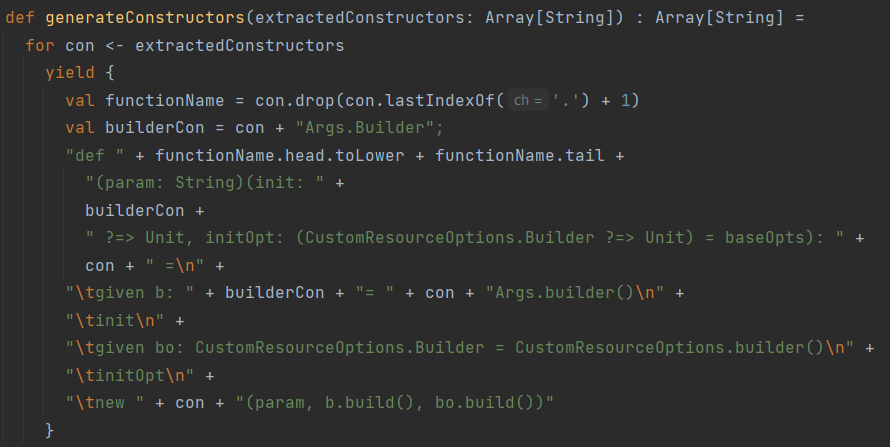
\includegraphics[width=1\columnwidth]{case_study/template_gen} 
  \captionof{figure}{Constructors generation}
\end{center}\mbox{}\\
The template is filled with the variables that represent the name of the constructors, and this is done for each constructor that has been found.\\
Since also the other functions are similar to this one, won't be reported here.

\subsubsection{The automatically generated syntactic sugar code}
Since the generated files contains many hundreds of lines of code, I'll report here only some samples of each file.\\

\paragraph{PulumiBuilderUtilFunctionsForScala}
First we have some default imports:
\begin{center}
  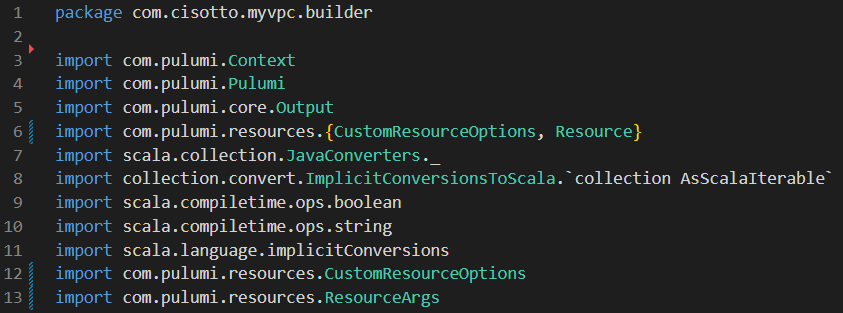
\includegraphics[width=1\columnwidth]{case_study/build_imports} 
  \captionof{figure}{Default import}
\end{center}\mbox{}\\
Then we have some all the generated union types, that look like:
\begin{center}
  \hspace*{-3cm}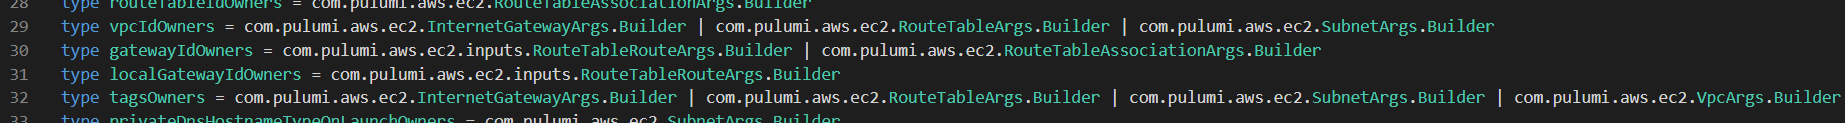
\includegraphics[width=1.5\columnwidth]{case_study/generated_union_types} 
  \captionof{figure}{Generated union types}
\end{center}\mbox{}\\
The implicit conversion functions are then printed:
\begin{center}
  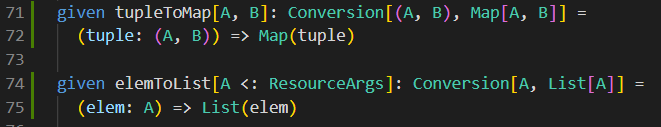
\includegraphics[width=1\columnwidth]{case_study/implicit_conv_fun} 
  \captionof{figure}{Implicit conversion functions}
\end{center}\mbox{}\\
Finally we have all the builders' methods that we encountered during our visit of the files with the JavaParser project:
\begin{center}
  \hspace*{-3cm}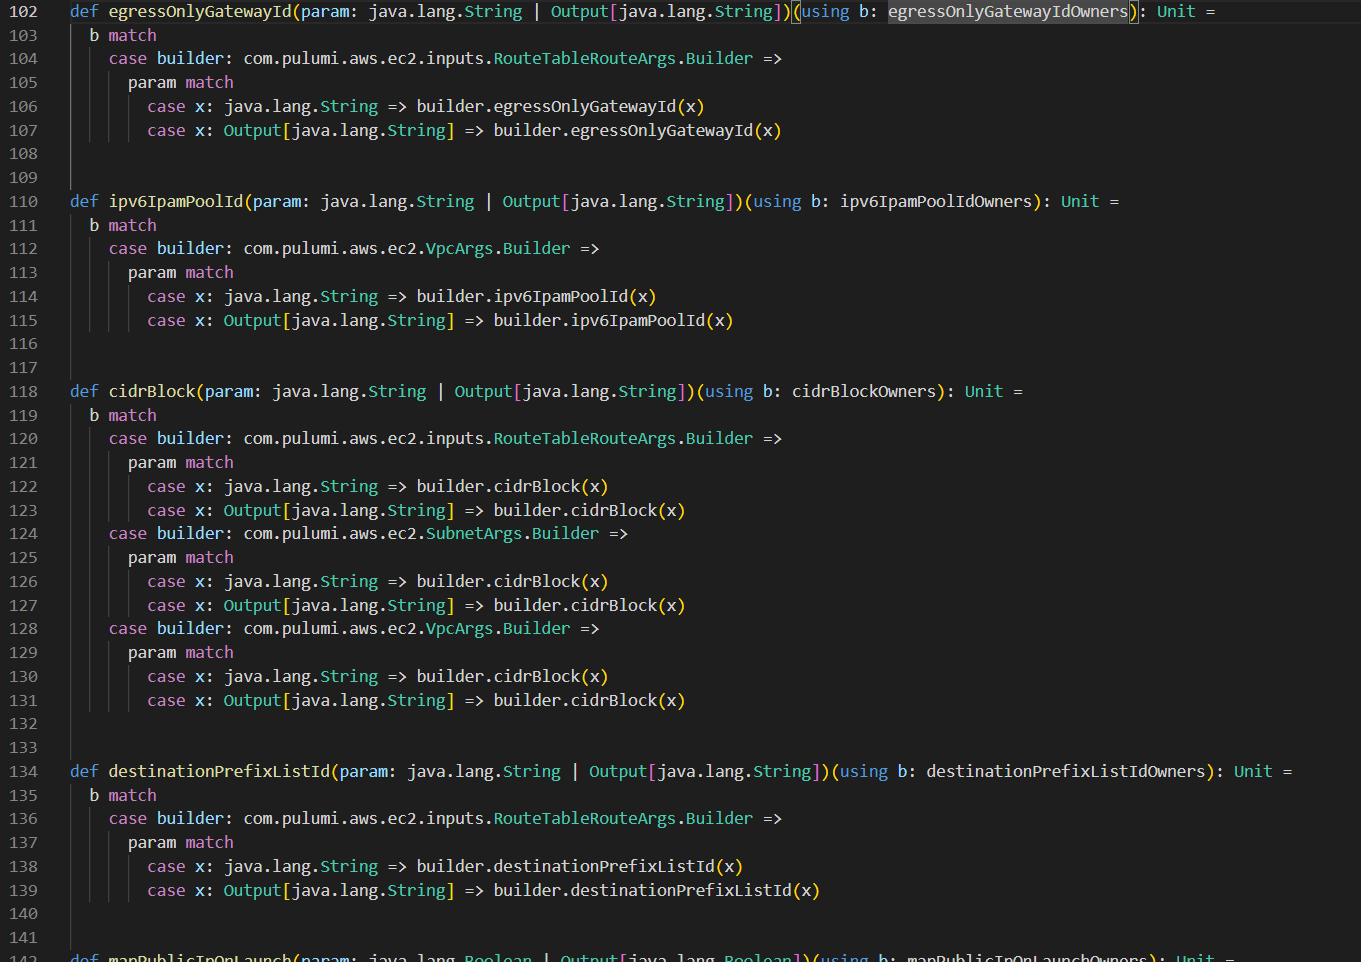
\includegraphics[width=1.4\columnwidth]{case_study/generated_builder_methods} 
  \captionof{figure}{Generated builders' methods}
\end{center}\mbox{}\\

\paragraph{PulumiUtilFunctionsForScala}
Also here we start with some default imports, then we have the baseOpts function and then all the constructors for the various resources:
\begin{center}
  \hspace*{-3cm}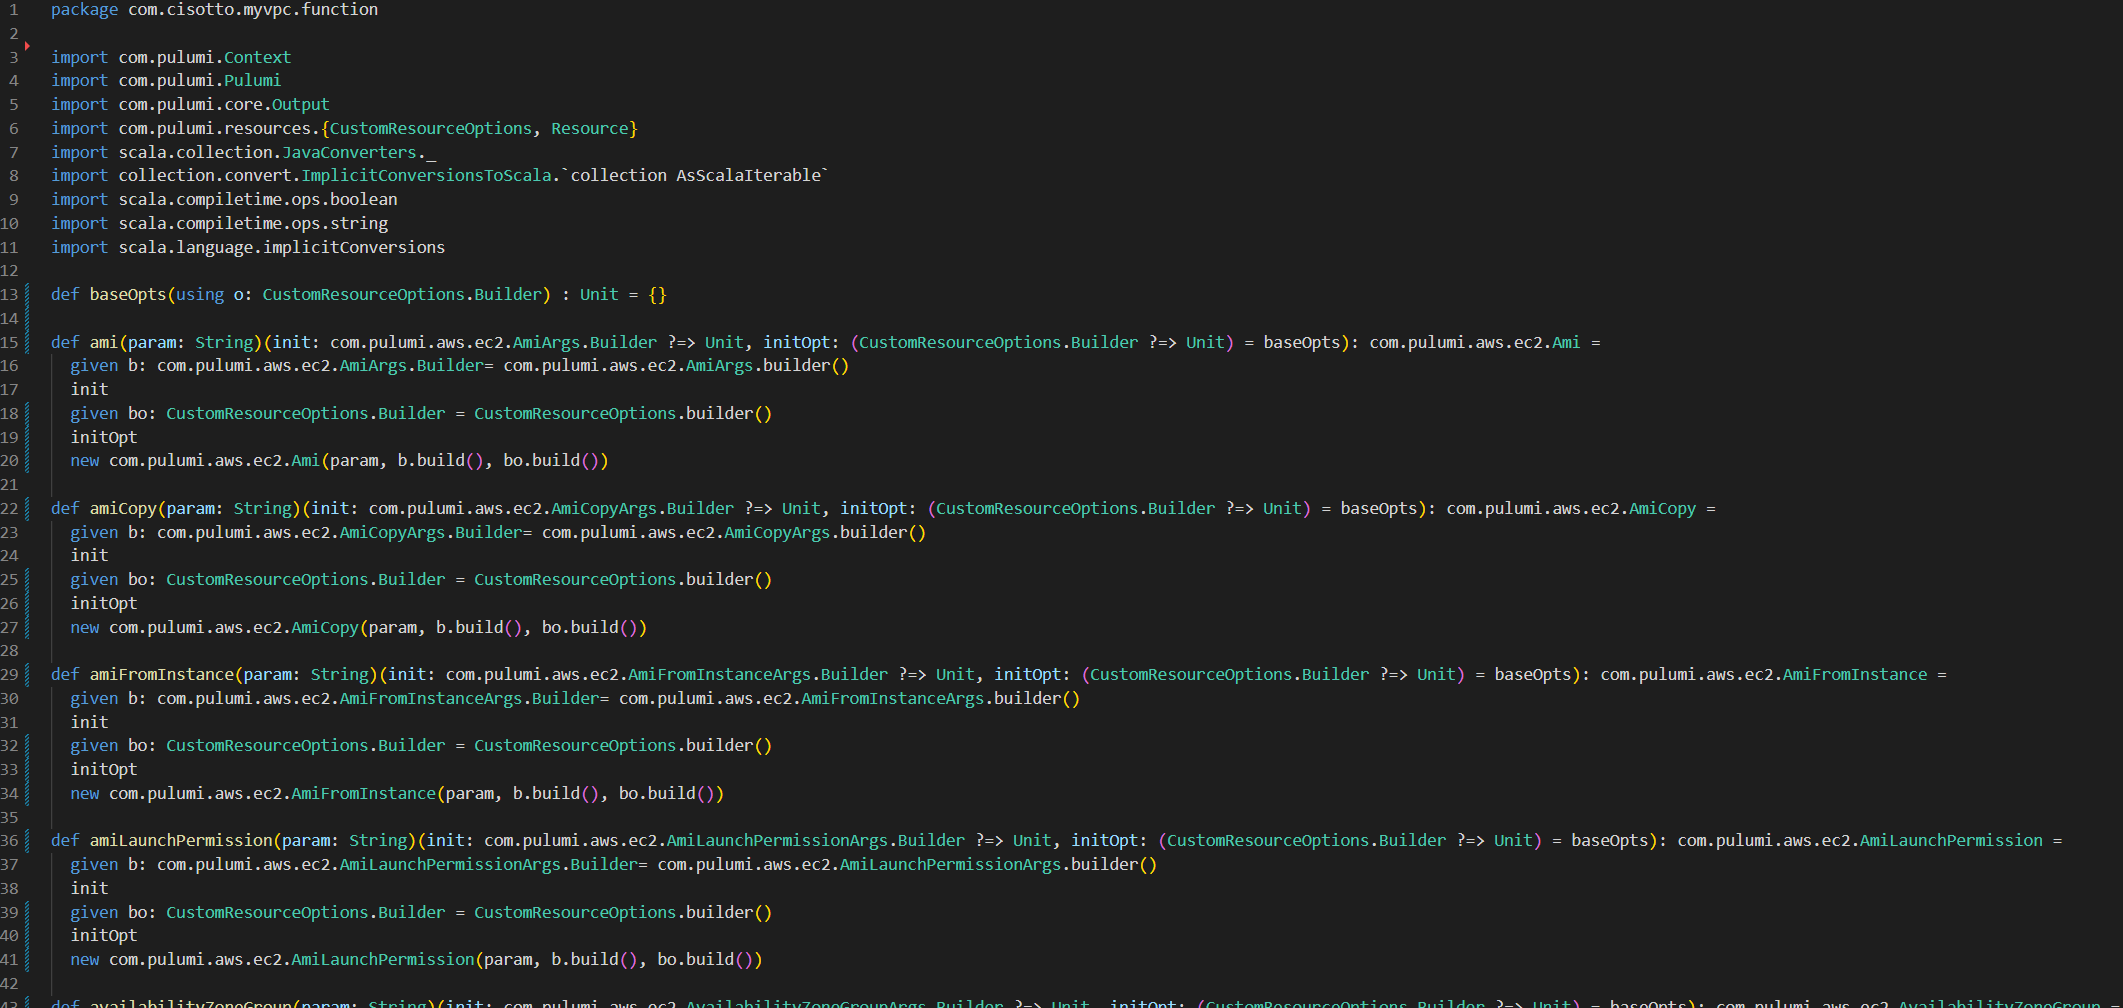
\includegraphics[width=1.4\columnwidth]{case_study/generated_constructors} 
  \captionof{figure}{baseOpts function and generated constructors}
\end{center}\mbox{}\\

\paragraph{Final observations on the generated code}
The builders' methods are really similar to each other, but they are not all following the same exact pattern across the whol AWS EC2 module.
Due to this fact, the generation of the code was affordable for the resources used in the case study, but to cover some corner cases for the rest of the resources some extra work both for the parser and for the algorithm that fills in the template would have been required.
Because of lack of time and since was not the final aim of the thesis to develop a complete support of Scala for all the AWS EC2 module, only the partial support for the used resources has been generated.\\
The constructors, instead, are all similar to each other and a complete support for AWS EC2 has been generated.
% !TEX encoding = UTF-8
% !TEX TS-program = pdflatex
% !TEX root = ../tesi.tex

%**************************************************************
\chapter{Comparison between the languages for Pulumi and the advantages of Scala}
\label{cap:comparisons}
%**************************************************************

\intro{Here all the advantages and disadvantages detected while using Typecript and Scala for our case study will be presented.}\\

%**************************************************************
\section{Code readability in Typescript vs in Scala}

\subsection{Readability in Typescript}
Typescript is less verbose than many other programming languages.
In the implementation we can appreciate how the passing of the builders methods' parameters have been achieved in a concise way using the JSON format.
This is fitting very well in a declarative approach and is very readable and intuitive, but some lacks of the language caused the code to lose readability and conciseness.

\subsubsection{Less readable code with pulumi.all and .apply}
\label{sssec:ts-subnets-comparison}
Lets consider once again the Typescript version of the function that is responsible for creating the subnets across the various availability zones:
\begin{center}
  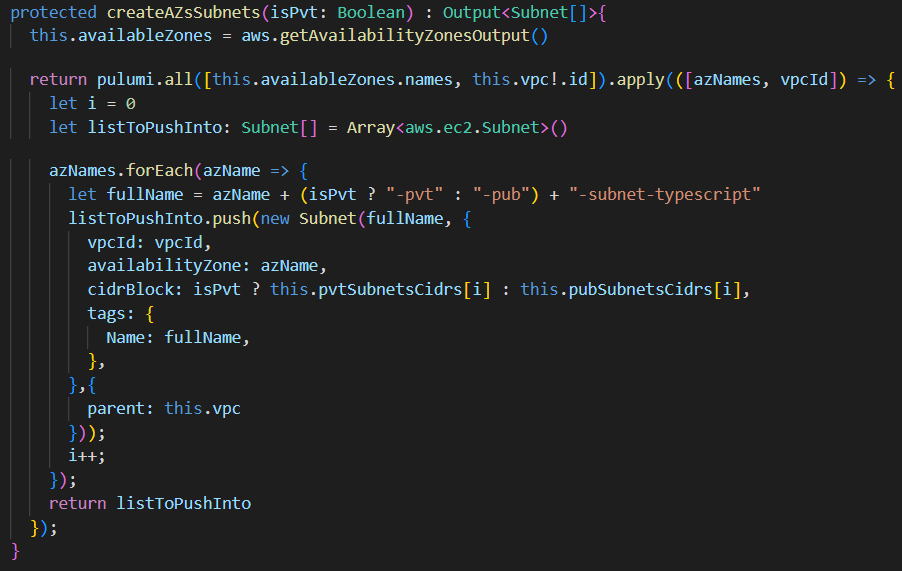
\includegraphics[width=1.0\columnwidth]{comparisons/ts_create_subnets} 
  \captionof{figure}{Typescript subnets creation}
\end{center}\mbox{}\\
When talking about readability, the \texttt{pulumi.all} and the \texttt{apply} functions are quite cryptic.
It takes us a little time to understand what are the return types of the \texttt{pulumi.all} and of the \texttt{apply} functions.
I remind here that the types of these two functions are fully explained in the \hyperref[par:ts-lambda]{The apply's lambda} paragraph.\\
We'll make furthers considerations on this function in the \hyperref[sssec:readability-for-yield]{Readability of the Scala's for yield vs pulumi.all and .apply} paragraph.

\subsection{Readability in Scala}
Also in Scala, thanks to the syntactic sugar used, we achieved a surprisingly readable code while defining the resources to be created on our Pulumi stack.

\subsubsection{Function currying}
The currying of Scala used to define our \textit{sugarized} functions granted us the possibility to declare the resources with this syntax:
\begin{verbatim}
  val resourceName = sugarizedResourceConstructor("res-name") {
    firstParameter(...)
    secondParameter(...)
    ...
  }
\end{verbatim}\mbox{}\\
This code is really readable (it resembles to a function definition) and is perfectly fitting in a declarative approach since we can have a straight list of the parameters we want to set for our resource.\\

\subsubsection{Hidden builders}
Thanks to the \texttt{given} and \texttt{using} keywords, builders aren't manually instantiated and we don't require to explicitly say on which builder instance we are calling the builders' methods.
This is letting us have an even more lightweight code that is really just focusing on what we need to instantiate instead of the how we could instantiate it.
Let's consider the VPC creation in our Scala solution and how would it is it created instead in a Java solution.\\
Scala solution:
\begin{lstlisting}[numbers=left, numberstyle=\tiny, numbersep=-5pt, stepnumber=1]
  val myVpc = vpc("scala-main") {
    cidrBlock("10.136.0.0/24")
    tags("Name" -> "myVpcScala")
  }
\end{lstlisting}\mbox{}\\
Java solution:
\begin{lstlisting}[numbers=left, numberstyle=\tiny, numbersep=-5pt, stepnumber=1]
  protected Vpc vpc = new Vpc("my-vpc-java", VpcArgs.builder()
    .cidrBlock("10.136.0.0/24")
    .instanceTenancy("default")
    .tags(Map.of("Name", "myVpcJava"))
    .build(),
          CustomResourceOptions.builder()
                  .parent(this)
                  .build());
\end{lstlisting}\mbox{}\\
Even if our syntactic sugar is using the very same APIs used from the Java's solution, the readability and the conciseness are entirely on another level.

\subsubsection{Implicit conversion functions to get rid of Map and List constructors while passing a single value}
The implicit conversion functions presented in the \hyperref[sssec:implicit-converion-functions]{Implicit conversion functions} paragraph let us get rid of the constructor of the Map and of the List if we're interested in passing a single value.\\
It is common, while declaring a new resource, to pass a single parameter to a builder's method that is actually expecting a list or a map of parameters.
In such cases the following syntax could be annoying:
\begin{center}
  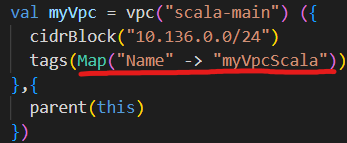
\includegraphics[width=0.7\columnwidth]{comparisons/explicit_map} 
  \captionof{figure}{Singleton map for a parameter}
\end{center}\mbox{}\\
%Tags expects a \texttt{Map[String, String]} value, but if we want to pass a single map element, we would appreaciate to get rid of the Map constructor and just write \texttt{"Name -> "myVpcScala"}.
But thanks to the implicit conversion functions the final result, as we have seen, is the desired one:
\begin{center}
  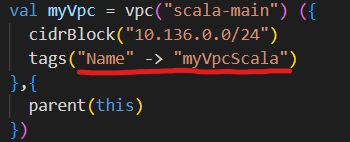
\includegraphics[width=0.7\columnwidth]{comparisons/implicit_map} 
  \captionof{figure}{Tuple for a parameter}
\end{center}\mbox{}\\
For a single parameter the difference of effort in explicitly writing the map constructor can be negligible, but when it comes to define many resources that use multiple methods that accept collections as input parameters, such a feature can really save us a lot of keystrokes, while keeping our code more readable and simple.

\subsubsection{Readability of the Scala's for yield vs pulumi.all and .apply}
\label{sssec:readability-for-yield}
Lets consider the function that creates the subnets.
With respect to the Typescript solution, the Scala one is more readable:
\begin{center}
  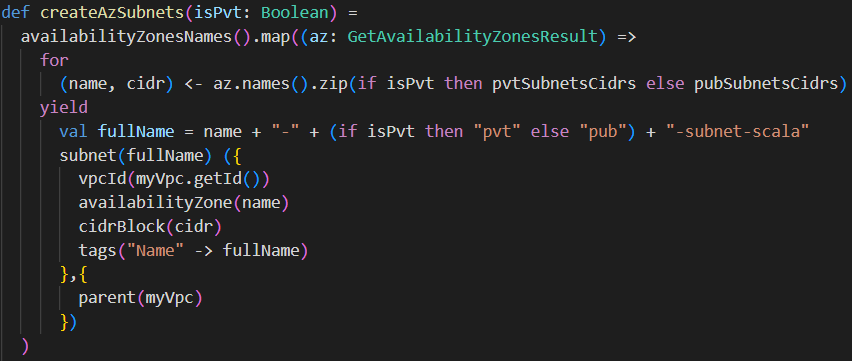
\includegraphics[width=1.0\columnwidth]{comparisons/scala_create_subnets} 
  \captionof{figure}{Scala subnets creation}
\end{center}\mbox{}\\
First, the \texttt{map} function is much more intuitive with respect to the \texttt{pulumi.all} and \texttt{apply} combination in the \hyperref[sssec:ts-subnets-comparison]{Typescript implementation}.
Moreover, the for comprehension used in the Scala version is a more elegant and concise solution.
In fact, the map function is doing the work of both the \texttt{pulumi.all} and \texttt{apply} functions, with much less code and in a much more readable way.\\
Furthermore, with Scala we're using the language feature of the for comprehension to automatically create a collection of the generated subnets and return them all together.\\
Differently, Typescript implementation requires us to explicitly insert the generated subnets in a variable as a side effect of the \texttt{foreach}.
Moreover, with Typescript, we also have to explicitly return the list at the end of the \texttt{apply}'s lambda.


\section{Expressiveness in Typescript vs in Scala}

\subsection{pulumi.all and .apply vs for comprehension and monads}

\subsubsection{Typescript compensate for its lack of expressiveness with the pulumi.all function}
In the \hyperref[sssec:pulumi-all]{pulumi.all} paragraph of the subnets creation section, we have seen how the concatenation of \texttt{apply} to the \texttt{pulumi.all} function let us create the subnets across the various availability zones.
Anyway, The process of wrapping two different \texttt{Ouptut} values in a single \texttt{Output} using the \texttt{pulumi.all} function, and then extract that newly created value form the \texttt{Output} context is verbose and complex.\\
Now, the \texttt{pulumi.all} function is effective but its existence is required to compensate for the lack of expressiveness of the Typescript language.

\subsubsection{Scala's expressiveness let us get rid of pulumi.all}
The functional nature of the Scala language let us get rid of the \texttt{pulumi.all} function thanks to the monad implementation for the \texttt{Output} type.
The \texttt{apply} function became the actual implementation of the \texttt{flatMap} function for the \texttt{Output[Monad]}.
The \texttt{map} function that we used in our function for the \hyperref[sssec:subnets-creation]{subnets creation} has been implemented only on the bases of the \texttt{flatMap} function.
So, we replaced the \texttt{pulumi.all} function with the \texttt{map} function offered by the \texttt{Monad[Output]}, and the \texttt{apply} function is now hidden behind the \texttt{map} implementation.\\
This achievement is perfectly depicting how the expressiveness of Scala permitted us to satisfy our need of applying functions on values contained inside a context (\texttt{Output} in our case), without resorting to an ad-hoc function created only for that specific purpose.
In fact, we would be able to implement a monad for any context type, while \texttt{pulumi.all} is working exclusively with the \texttt{Output} type.
Moreover, the \texttt{map} function is much more intuitive to an user rather than the \texttt{pulumi.all} and the explicit \texttt{apply} functions.

%On the other hand, when we have to combine two values of different \texttt{Output}s types in another value of another \texttt{Output} type, we must rely on the \texttt{pulumi.all} and \texttt{.apply} functions.
%In the \hyperref[sssec:pulumi-all]{pulumi.all} paragraph we have seen how such a function is used in the Typescript implementation to create the subnets in our availability zones.


%Now, if we want to use the \texttt{.apply} function to 
%since we have to pass through a pulumi.all to wrap the availability zones names \texttt{Output<String[]>} and the 


%\subsubsection{Poor tools to act on groups of Outputs}

%\section{Java solution observations}

%\subsection{Advantages of using Pulumi's Java APIs}

%\subsection{Disadvantages of using Pulumi's Java APIs}

%\subsubsection{Verbose code}

%\section{My Scala solution observations}

%\subsection{Advantages of using my Scala syntactic sugar}

%\subsubsection{Very concise code}

%\subsubsection{Very readable and elegant code}

%\subsubsection{More powerful constructs thanks to the for-comprehension and the monads to act on groups of Outputs}

%\subsection{Disadvantages of using my Scala syntactic sugar}

%\subsubsection{Partial solution, not all the corner cases have been considered}

%\section{Final thoughts on the Scala solution}

%**************************************************************
% Materiale finale
%**************************************************************
\backmatter
\printglossaries
% !TEX encoding = UTF-8
% !TEX TS-program = pdflatex
% !TEX root = ../tesi.tex

%**************************************************************
% Bibliografia
%**************************************************************

%\cleardoublepage
\chapter{Bibliografia}

\nocite{*}
% Stampa i riferimenti bibliografici
\printbibliography[heading=subbibliography,title={Riferimenti bibliografici},type=book]

% Stampa i siti web consultati
\printbibliography[heading=subbibliography,title={Siti web consultati},type=online]
\end{document}
